%!TEX root = alicepreprint_CDS.tex

%% \ask{General Jana/MP: need to rework the figures (symbols;colors etc); english: decide on the tense.}

\section{Introduction}
%%\ask{Intro taken from the ID spectra mult dependence in p-Pb. Needs adjustments for the purpose of this paper.}

High--energy heavy ion collisions provide a unique opportunity to study properties of hot and dense QCD medium composed of deconfined partons - the quark--gluon plasma (QGP).
The QGP is predicted by the lattice QCD calculations \cite{Satz:2000bn,Bass:1998vz,Shuryak:1984nq,Cleymans:1985wb}.
The cross-over transition from hadronic matter to the QGP matter at zero baryochemical potential is expected to take place once the temperature of the matter $T$ reaches values of about $T_{\it{c}} = 150~\mev$ and/or energy density $\epsilon_{c}$ of about 0.5 GeV/fm$^3$ \cite{Borsanyi:2010cj,Bhattacharya:2014ara}.
The measurements indicate that the most violent collisions of lead ions at the Large Hadron Collider (LHC) at centre-of-mass energy per nucleon--nucleon collision \sqrtsnn{2.76}\ create conditions well above the critical temperature at approximately zero baryochemical potential.
The bulk matter created in those collisions can be quantitatively described in terms of relativistic hydrodynamics and statistical hadronization models.
The initial hot and dense partonic matter rapidly expands and cools down, ultimately undergoing a transition to a hadron gas phase~\cite{Muller:2006ee}.
During the expansion phase, collective hydrodynamic flow develops from the initially generated pressure gradients in the strongly interacting system.
This results in a characteristic dependence of the shape of the transverse momentum (\pt) distribution on the particle mass that can be described using a common kinetic freeze-out temperature parameter \Tfo\ and a collective average expansion velocity \avbT~\cite{Schnedermann:1993ws}.

The interpretation of heavy-ion results requires the understanding of results from smaller collision systems such as proton--proton (\pp) or proton--nucleus (pA).
%%Proton-nucleus collisions are intermediate between proton--proton and nucleus-nucleus collisions in terms of system size and number of produced particles.
Comparisons of particle production in pp, pA, and AA reactions has frequently been used to separate initial state effects, linked to the use of nuclear beams or targets, from final state effects, associated to the presence of hot and
dense matter.
%%At the LHC, however, the pseudorapidity density of final state particles in pA collisions reaches values comparable to semi-peripheral Au--Au ($\sim$60\% most central) and Cu--Cu ($\sim$30\% most central) collisions at top Relativistic Heavy-Ion Collider (RHIC) energy~\cite{Alver:2010ck}.
However, the measurements at the LHC in high-multiplicity pp and \pPb\ collisions have revealed unexpectedly strong long-range correlations of produced particles \cite{Khachatryan:2010gv,CMS:2012qk,Abelev:2012ola,Aad:2012gla,Aad:2013fja,Chatrchyan:2013nka} falsifying the assumption that final state effects can be neglected in pA.
Moreover, measurements of identified-hadron production \cite{Abelev:2013haa} have shown qualitatively similar features as in AA collisions \cite{Abelev:2013xaa,ABELEV:2013wsa}.
In particular, the ratio of baryon and meson transverse momentum (\pt) spectra shows a pronounced maximum at intermediate ($2-5$~\gevc) \pt~\cite{Abelev:2013haa}.
The \pt\ dependence of the ratio has been discussed in terms of an interplay between the radial expansion of the system and particle production within a common velocity field (collective flow)~\cite{Schnedermann:1993ws}, soft-hard parton recombination \cite{Fries:2003vb} and high-energy parton shower (jet) hadronization at high \pT.
On the other hand, the measurements of inclusive jet production at mid-rapidity in pA collisions \cite{Adam:2015hoa,Adam:2015xea} show that the initial state nuclear effects such as shadowing and gluon saturation (CGC) \cite{McLerran:2001sr,Salgado:2011wc}, or multiple scatterings and hadronic re-interactions in the initial and final state \cite{Krzywicki:1979gv,Accardi:2007in} are negligible as compared to the same measurements in \pp\ collisions.
In particular, the suppression related to the creation of the QGP in AA collisions was not observed in \pPb\ collisions \cite{Aad:2010bu,Chatrchyan:2012nia,Aad:2012vca,Abelev:2013kqa,Aad:2014bxa}.
%%Various mechanisms have been proposed to explain the origin of this collective particle production.
%%Both a Color Glass Condensate (CGC) description~\cite{Dusling:2013oia}, based on initial state nonlinear gluon interactions, as well as a model based on hydrodynamic flow~\cite{Bozek:2012gr,Qin:2013bha}, assuming strong interactions between final state partons or hadrons, can give a satisfactory description of the \pPb\ correlation data.
%%However, the modeling of small systems such as \pPb\ is complicated because uncertainties related to initial state geometrical fluctuations play a large role and because viscous corrections may be too large for hydrodynamics to be a reliable framework~\cite{Bzdak:2013zma}.

In this letter we report on the measurement of \lda, \alda\ and \ks\ where their production is studied separately within the region associated to a hard scattering and the remainder of the event (the so called ``underlying event''). The hard scatterings are tagged by selecting a jet ($\ptjet > 10$ or $20~\gevc$) reconstructed using charged particles with the anti-\kt\ algorithm with the resolution parameter $R=0.2$, $0.3$ and $0.4$. The \lda/\ks\ ratio associated to jets is reported as a function of particle \pt\ and as a function of their distance to the jet axis.
% and for a selection of the event multiplicity classes of the \pPb\ collisions.

%%%%%%%%%%%%%%%%%%%%%%%%%%%%%%%%%%%%%%%%%%%%%%%%%%%%%%%%%%%%%%%%%%

\section{Data analysis}

\subsection{Data sample and detector description}

The data used in this analysis was recorded by the ALICE detector~\cite{Aamodt:2008zz} during the LHC p--Pb run at \sqrtsnn{5.02} in the beginning of $2013$. Since the ``two-in-one'' magnet design of the LHC~\cite{Evans:2008zzb}, the energies of the two beams are not independent and their ratio is fixed to equal to the ratio of the charge/mass ratios of each beam. Consequently, the nucleon--nucleon centre-of-mass system (cms) was shifted by a rapidity of $\Delta y_{\rm NN}=0.465$ in the direction of the proton beam. The analyzed data was collected for the beam configuration, in which the Pb beam circulated in the ``counter-clockwise'' direction traveling from negative to positive rapidity.
%%The number of colliding bunches was varied from $8$ to $288$. The total number of proton and Pb ion bunch intensities ranged from $0.2\times 10^{12}$ to $6.5\times 10^{12}$ and from $0.1\times 10^{12}$ to $4.4\times 10^{12}$, respectively.
%%The luminosity at the ALICE interaction point for the data used in this analysis was up to $5\times 10^{27}$~cm$^{-2}$s$^{-1}$ resulting a $10$~kHZ hadronic interaction rate. The r.m.s of the interaction region is $6.3$~cm along the beam direction and $60~\mu{\rm m}$ in the direction to the transverse to the beam. The used data was collected for the beam configuration, in which the Pb beam circulated in the ``counter-clockwise'' direction, corresponding to travel from ALICE C to A side or positive rapidity.

The ALICE apparatus described in detail in \cite{Aamodt:2008zz} consists of central barrel detectors covering the pseudo-rapidity interval $|\hlab|<0.9$, a forward muon spectrometer covering $-4.0<\hlab<-2.5$, and a set of detectors at forward and backward rapidities used for triggering and event characterization.
%%In this analysis the V0 detector system~\cite{Abbas:2013taa} was used for triggering.
%% and for estimating the multiplicity of charged particles in the forward rapidity region
%%V0 consists of two arrays of 32 scintillator tiles each, placed around the beam vacuum tube on either side of the interaction region at $z =-90$ cm and $z=+340$ cm.
%%The two arrays cover the pseudo-rapidity intervals $-3.7 < \hlab < -1.7$ (V0C) and $2.8 < \hlab < 5.1$ (V0A), respectively.
The data presented in this letter were recorded using the minimum bias trigger provided by the V0 detector system \cite{Abbas:2013taa} consisting of two arrays of 32 scintillator tiles each, placed around the beam vacuum tube on either side of the interaction region covering the pseudo-rapidity intervals $2.8 < \hlab < 5.1$ (V0A) and $-3.7 < \hlab < -1.7$ (V0C).
%%The minimum-bias trigger signal was provided by the V0A and V0C sets of scintilator tiles~\cite{Abbas:2013taa}.
%%The signal amplitude and arrival time collected in each tile of the detectors were recorded.
A coincidence of signals in both V0A and V0C was required to remove contamination from single diffractive and electromagnetic events~\cite{ALICE:2012xs}.
%%The resolution of the arrival time is better than $1$~ns, allowing discrimination of beam--beam collisions from background events produced outside of the interaction region.
In addition two neutron Zero Degree Calorimeters (ZDCs) located at $+112.5$ m (\ZNA) and $-112.5$ m (\ZNC) from the interaction point were used for beam background rejection. % and an alternative estimator of the event activity.
%%In the offline analysis, background was further suppressed by the time information recorded in two neutron Zero Degree Calorimeters (ZDCs), which located at $+112.5$~m (ZNA) and $-112.5$~m (ZNC) from the interaction point.
A dedicated quartz radiator Cherenkov detector (T0)~\cite{Akindinov:2013tea} provided the measurement of the event time of the collision.

%%In order to reduce the underlying background of jets and improve the resolution of the $\Vzero$ decay vertices, the pileup and bad quality events are rejected by the vertex quality cuts.
%%In addition to the trigger selection, timing and vertex-quality cuts were used to suppress pile-up events and retain only beam-beam collisions.

Tracking and particle identification were performed using the information provided by the Inner Tracking System (ITS) \cite{Aamodt:2010aa}, the Time Projection Chamber (TPC) \cite{Alme:2010ke} and the Time Of Flight (TOF) \cite{Akindinov:2013tea} detectors, that have full azimuthal coverage in the pseudo-rapidity interval $|\hlab|<0.9$.
These central barrel detectors are located inside a large solenoidal magnet, which provides a magnetic field of 0.5 T along the beam direction ($z$ axis in the ALICE reference frame).

%%The detector closest to the beam axis is the Inner Tracking System (ITS).
The ITS is composed of six cylindrical layers of silicon detectors, with radial distances from the beam axis ranging from 3.9~cm to 43.0~cm.
The two innermost layers, with average radii of 3.9~cm and 7.6~cm, are equipped with Silicon Pixel Detectors (SPD) covering the pseudo-rapidity ranges of $|\hlab|< 2.0$ and $|\hlab|< 1.4$, respectively.
The two intermediate layers are made of Silicon Drift Detectors (SDD), while Silicon Strip Detectors (SSD) equip the two outermost layers.
The high spatial resolution of the silicon sensors, together with the low material budget (on average 7.7\% of a radiation length for tracks crossing the ITS perpendicularly to the detector surfaces, i.e.\ $\hlab=0$) and the small distance of the innermost layer from the beam vacuum tube, allow for the measurement of the track impact parameter $d_{\rm DCA}$ in the transverse plane.
The $d_{\rm DCA}$ is defined by the distance of closest approach (DCA) of the track to the primary vertex in the plane transverse to the beam direction, and is measured with a resolution better than
\SI{75}{\micro\metre}
%%${\mathrm \mu m}$
for transverse momenta $\pt>1~\gevc$~\cite{Aamodt:2010aa}.
%%The SPD provides also a measurement of the multiplicity of charged particles produced in the collision based on track segments (tracklets) built by associating pairs of hits in the two SPD layers.
The events were further selected by requiring a reconstructed vertex within $10$~cm ($v_{z}<10$~cm) along beam axis and that the vertices built from SPD tracklets and from the global tracks (combining information of ITS and TPC) were compatible.
The analysis required a reconstructed vertex, which was the case for 98.2\% of the events selected by the trigger. The total number of events retained in the analysis was $96\cdot10^{6}$.

At larger radii ($85<r<247~\cm$), a 510 cm long cylindrical TPC provides track reconstruction with up to 159 three-dimensional space points per track, as well as particle identification via the measurement of the specific energy deposit $\dedx$ in the gas.
%% The charged particle identification capability of the TPC is supplemented by the TOF, which is equipped with Multi-gap Resistive Plate Chambers  (MRPCs) located at radial distances between 377 and 399 cm from the beam axis. The overall TOF resolution including the uncertainty on the time at which the collision took place, and the tracking and momentum resolution was about 160~ps for the data-taking period considered in this analyses.

%%%%%%%%%%%%%%%%%%%%%%%%%%%%%%%%%%%%%%%%%%%%%%%%%%%%%%%%%%%%%%%%%%%%%

\subsection{Charged-particle and jet reconstruction}

%%The spectrum of jets reconstructed with charged particles in \pPb\ collisions at \sqrtsnn{5.02} within ALICE was reported in \cite{Adam:2015hoa}.
The charged-particle and jet reconstruction in this letter follows the analysis described in detail in \cite{Adam:2015hoa}. Here only a brief review of the most relevant points is discussed.
Charged-particle tracks reconstructed in the ITS and the TPC with $\pt > 0.15~\gevc$~and within a pseudorapidity interval $|\eta_\mathrm{lab}|<0.9$ that satisfied a DCA requirement
%s of the distance of closest approach (DCA) to primary vertex
$d_{\rm DCA} < 2.4$~cm were used as input to the jet reconstruction.
The azimuthal distribution of these high quality tracks is not completely uniform due to inefficient regions in the SPD. This was compensated by considering in addition tracks without reconstructed track points in the SPD.
To improve the momentum resolution for those tracks, the primary vertex was used as an additional constraint in the track fitting.
This approach yields a uniform tracking efficiency within the acceptance, which is needed to avoid geometrical biases in the jet reconstruction that can be caused by an unphysical non-uniform density of reconstructed tracks.
The procedure is described in detail in the context of jet reconstruction in \cite{Adam:2015hoa}.
For the analyzed data, the additional tracks (without SPD track points) constitute approximately 4.3\% of the used track sample. The overall efficiency for charged particle detection, including the effect of tracking efficiency as well as the geometrical acceptance, is 70\% at $\pt = 0.15~$\gevc\ and increases to 85\% at $\pt = 1~$\gevc\ and above.

The jets were reconstructed using the anti-$\kT$ algorithm~\cite{Cacciari:2008gp} from the FastJet package~\cite{Cacciari:2011ma,Cacciari:2005hq} with resolution parameters of $R=0.2$, $0.3$ and $0.4$.
Only the jets where the jet-axis was found within the acceptance window $\abs{\hlab}<0.35$ that is fully overlapping with the acceptances of both charged particle tracks ($\abs{\hlab}<0.9$) and the weakly decaying particles ($\Vzero$s) ($\abs{\hlab}<0.75$) for any of the jet resolution parameters.
The jet transverse momentum is calculated by FastJet using the \pt\ recombination scheme.

In general the transverse momentum density of the background originating from the underlying event and/or pile-up (particles not associated to the hard scattering) contributes to the jet energy reported by the jet finder.
The correction of the jet energy scale accounting for the background energy can be estimated on event-by-event basis using the median of all jet candidate clusters $\ptch$ reconstructed with the $\kt$ algorithm per unit area \cite{Cacciari:2008gn}.
This method has been used in the analysis of \PbPb\ events \cite{Abelev:2013kqa,Adam:2015ewa}.
In this analysis, an estimate adequate for the more sparse environment of $\pPb$ collisions was employed \cite{Adam:2015hoa}. The resulting mean of the background \pt\ density $\avg{\rho^{\rm ch}}=1.02~\pm~0.91~\GeVc~{\mathrm{rad}}^{-1}$ for unbiased events and, $\avg{\rho^{\rm ch}}=2.2~\pm~1.47~\GeVc~{\mathrm{rad}}^{-1}$ for events containing a jet with $\ptchraw>20~\GeVc$~\cite{Adam:2015hoa}.

%%The correction of the jet transverse momentum ($\pT[jet]^{\rm ch}$) scale accounting for the transverse background energy density, $\rho^{\rm ch}$, which can be estimated on event-by-event basis using the median of all jet candidate clusters $\pT$ reconstructed with the $\kT$ algorithm per unit area~\cite{Cacciari:2007fd,Abelev:2013kqa},
%%\begin{equation}
%%\pT[jet]^{\rm ch}=\pT[jet]^{\rm ch,raw}-\rho^{\rm ch}A_{\rm jet}^{\rm ch},
%%\end{equation}
%%where,~  $A_{\rm jet}^{\rm ch}$  and $\pT[jet]^{\rm ch,raw}$ are the measured area~\cite{Cacciari:2008gn} and transverse momentum for the charged particle jets.
%%To further correct the fluctuations, caused by the more sparse environment of p--Pb events, of background density, an approach described in~\cite{Chatrchyan:2012tt} was employed.

%%\ask{We need to comment on: a) the jet efficiency for $\pt < 20~\gevc$. Not in the cited paper. Below some text from the jet in \pPb\ paper.}

The resulting kinematic efficiency for generator level jets was established using using PYTHIA \cite{PYTHIA}. For jets of $\pt=10~\gevc$ it was about 65\% and 90\% for jets with $\pt =20~\gevc$.
%Reconstruction efficiency for jets with $\pt > 10~\gevc\ $ was greater than 95\%.

\subsection{Particle identification and \Vzero\ particle reconstruction}

Charged-hadron identification in the central barrel was performed with the ITS and TPC detectors. The drift and strip layers of the ITS provide a measurement of the specific energy loss with a resolution of about 10\%. In a standalone tracking mode, the identification of pions, kaons, and protons is thus extended down to respectively 0.1, 0.2, 0.3~\gevc\ in \pt. The TPC provides particle identification at low momenta via specific energy loss \dedx\ in the gas by measuring up to 159 samples per track with a resolution of about 6\%. The separation power achieved in \pPb\ collisions is identical to that in pp collisions~\cite{Abelev:2014ffa}.
%% Further outwards at about 3.7 m from the beam line, the TOF array allows identification at higher \pt\ measuring the particle speed with the time-of-flight technique. The total time resolution is about 85 ps for events in the multiplicity classes from 0\% to about $80$\%.  In more peripheral collisions, where multiplicities are similar to pp, it decreases to about 120 ps due to a worse start-time (collision-time) resolution~\cite{Abelev:2014ffa}. The start-time of the event was determined by combining the time estimated using the particle arrival times at the TOF and the time measured by the T0 detector.

%%Since the \pPb\ center-of-mass system is shifted in the laboratory frame with a rapidity of $\Delta y_{\rm NN}=0.465$, the nominal acceptance of the central barrel of the ALICE detector was asymmetric with respect to \ycms\ = 0.  In order to ensure good detector acceptance and optimal particle identification performance, tracks were selected in the rapidity interval $0 < \ycms < 0.5$ in the nucleon-nucleon center-of-mass system. Event generator studies and repeating the analysis in $\left|\ycms\right| < 0.2$ indicate differences between the two rapidity selections smaller than 2\% in the normalization and 3\% in the shape of the transverse momentum distributions.

%%%%%%%%%%%%%%%%%%%%%%%%%%%%%%%%%%%%%%%%%%%%%%%%%%%%%%%%%%%%%%%%%%%%%
%%\subsection{\lda\ (\alda) and \ks\ reconstruction}
%%\label{sec:V0Reco}
The $\Vzero$ particles, $\ks$ and $\lda$ ($\alda$), were identified exploring the characteristics of their weak decay topologies in the channels $\ks\to\pion^{+}\pion^{-}$ and $\lda(\alda)\to{\rm p}\pion^{-}(\pbar\pion^{-})$, which have branching ratios of $69.2\%$ and $63.9\%$, respectively~\cite{Agashe:2014kda}.
The reconstruction and the selection criteria of the \Vzero\ particles follow the analysis in \cite{Abelev:2013haa} with the exception of the rapidity selection of the particles and their decay products.
In particular, \pt-differential yields of \Vzero\ particles were extracted via the invariant-mass method described in \cite{Abelev:2013haa} but the $\Vzero$ decay-product tracks were selected in the acceptance window $\abs{\hlab}<0.8$, whereas only the \Vzero\ candidates found in $\abs{\hlab}<0.75$ were retained.
This ensured that the reconstruction efficiency was approximately constant throughout the selected pseudo-rapidity.
The topological selection of \Vzero\ candidates within the kinematic range of this analysis yielded an almost background-free invariant-mass spectra with the lowest signal/background ratio among all of the \Vzero\ particles still greater than 10.
%% \ask{MP: Sentence added on req. by Jana: ``add a description how the \lda\ and \kzero\ sample is clean after topological selection '' => check number - extract from the invariant-mass for the lowest pT bin considered - 0.5 \gevc.}
We note that due to the track selection optimized for weak decays only about 0.1\% of the \Vzero\ daughter tracks contribute to the charged-particle jet reconstruction.
%% \ask{more details needed?}

%%\as~k{stop h~ere - 5:20PM June 20}

%%%%%%%%%%%%%%%%%%%%%%%%%%%%%%%%%%%%%%%%%%%%%%%%%%%%%%%%%%%%%%%%%%%%%

\subsection{Matching of \Vzero\ particles to jets and underlying event}
\label{sec:c05V0JetMat}

%%In this~ analysis the selection criteria for primary charged particle tracks used for the jet reconstruction are different from those of the \Vzero\ candidate daughter tracks.
%%In this analysis that the selection cuts for primary particle tracks used for the jet reconstruction are not compatible with the \Vzero\ candidate tracks.
%%Only a small fraction (<1\%) of \Vzero\ candidate daughter tracks enter the jet reconstruction.
To obtain the yield of \Vzero\ particles within a jet cone the \Vzero\ particles are selected based on their distance from the jet centroid $R_{\Vzero-{\rm jet}}$ in the pseudo-rapidity and azimuthal angle plane ($\hlab \times \varphi)$) such that:
\begin{equation}
R_{\Vzero-{\rm jet}}=\sqrt{(\hlab^{\rm jet} - \hlab^{\Vzero})^{2} + (\varphi^{\rm jet} - \varphi^{\Vzero})^{2}}.
\end{equation}
A particle that is within the radius $R_{\Vzero-{\rm jet}} < R$ is considered matched to a given jet.
In \pPb\ collisions the probability for a particle with $\pT>0.5~\gevc$ to match to two jets with $\pt^{\mathrm{jet}} > 10~\gevc$ is significantly less than $1\%$
%%(\ask{check number})
and in these cases the higher-energy jet is preferred.
Moreover, removal of the events with two or more jets matching a single particle did not alter the result of the analysis.
The procedure for extraction of the yield of $\Vzero$ particles associated with a jet within a cone $R$ (JC $\Vzero$) can be summarized as follows.
The \Vzero\ candidates selected within the acceptance of $|\eta|<0.75$ were associated to the hard scattering with a distance cut in pseudo-rapidity and azimuthal angle plane $R_{\Vzero-{\rm jet}}<R$.
For each \pt\ interval the JC raw yield of \Vzero\ particles was established using the invariant-mass technique where the combinatorial background was interpolated from the side bands around the mass peak.
The mass peak is defined by the width and mean of the peak for the inclusive \Vzero\ candidates.
Then the raw JC yield can be corrected for the contribution of particles from the underlying event (UE).
The UE is simply defined as set of particles that is not associated to the hard scatterings tagged by the charged jets considered in this analysis.
%% (various estimators of \Vzero\ particles of the UE are discussed below). %in subsection \ref{sec:V0UE}).

%%\begin{figure}[]
%%\begin{center}
%%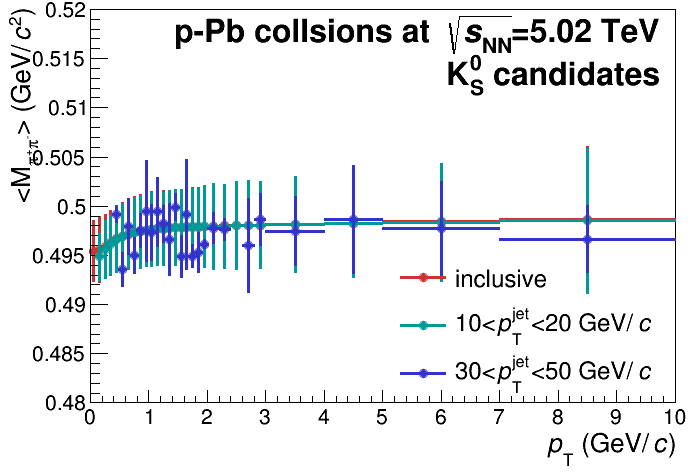
\includegraphics[width=.49\textwidth]{c02/KshortInvM}
%%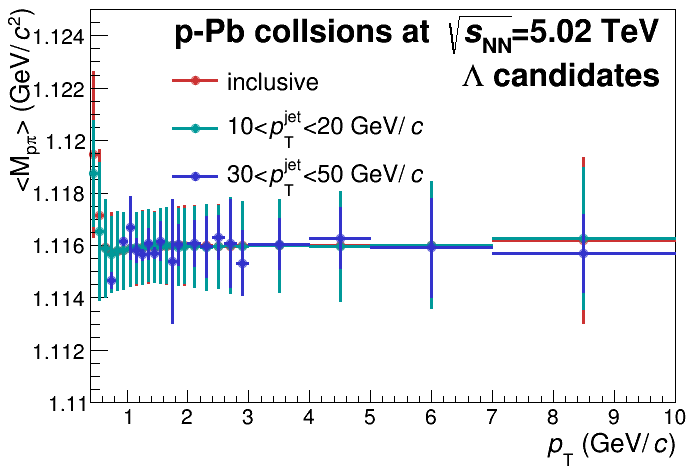
\includegraphics[width=.49\textwidth]{c02/LambdaInvM}
%%\caption{The mean and width of \Vzero\ invariant-mass distribution extracted
%%         by the Gaussian fit for the inclusive $\Vzeros$ candidates
%%         and JC $\Vzero$ candidates as a function of $\pT$ in data.}
%%\label{fig:V0FitInvM}
%%\end{center}
%%\end{figure}

%%Figure~\ref{fig:V0FitInvM} shows the comparison of the mean and width of \Vzero\ invariant-mass distribution extracted by the Gaussian fit for the inclusive \Vzeros\ candidates and JC \Vzero\ candidates as a function of $\pT$ in data.
%%The mean and width in the $\Vzero$ invariant-mass distributions for the inclusive \Vzeros\ and JC \Vzeros\ are compatible within statistical uncertainties.
%%To avoid statistic fluctuations found in high-\pT\ jet selection, the number of JC \Vzeros is extracted using the mean and width obtained in the inclusive $\Vzero$ invariant-mass distribution.

%%Given the track selection and the matching procedure the efficiency for finding a \Vzero\ within a jet is a product of single particle \Vzero\ efficiency and jet finding efficiency.

%%%%%%%%%%%%%%%%%%%%%%%%%%%%%%%%%%%%%%%%%%%%%%%%%%%%%%%%%%%%%%%%%%

%%\subsection{\Vzero\ particles from the underlying event}
%%\label{sec:V0UE}

To extract the UE yield of \Vzero\ particles several estimators have been investigated: i) {\it outside cone} (OC) selection composed of the \Vzero\ particles that were not matched to any jet considered in the analysis within events containing a jet such that $R_{\Vzero-{\rm jet}} > R_{\rm cut}$; ii) the {\it perpendicular cones} (PC) selection composed of the \Vzero\ particles found at azimuthal angles larger than $R_{\rm cut}$: $\Delta \varphi > R_{\rm cut}$, where $\Delta \varphi= \varphi^{\rm jet} - \varphi^{\Vzero}$; and iii)  %%\ask{(say the value)}
the {\it non-jet events} (NJ) selection composed of the \Vzero\ particles found in events that do not contain a jet with $\ptjet>5~\gevc$.

In practice, a useful quantity for performing the subtraction of the non-jet contribution of the \Vzero\ particles is their density per unit area
\begin{equation}
\rho^{\Vzero}(\pt) = N^{\Vzero}(\pt) / A^{\Vzero},
\label{eq:defv0rho}
\end{equation}
where $N^{\Vzero}$ is the number of particles and $A^{\Vzero}$ is the acceptance in pseudo-rapidity and azimuthal angle. Consequently, the number of the UE \Vzero\ particles within a jet can be calculated as $N=\rho^{\Vzero} \Ajet$ for each estimator separately.
%% In this analysis we consider the jet area $\Ajet = {\rm \pi} R^2$.
In general the density of \Vzero\ particles within jets (JC) can be defined as $\rhovzero_{\mathrm{JC}} = \rhovzero_{\mathrm{JC, raw}} - \rhovzero_{\mathrm{UE}}$, where $\mathrm{UE}$ can be any of the OC, PC, NJ background estimators.
In this analysis we choose PC as the default background estimator and use OC and NJ to quantify the systematic uncertainty.

%%%%%%%%%%%%%%%%%%%%%%%%%%%%%%%%%%%%%%%%%%%%%%%%%%%%%%%%%%%%%%%%%%
%%\subsection{\Vzero\ reconstruction efficiency}
\subsection{Corrections for finite \Vzero\ reconstruction efficiency and feed-down}
\label{sec:c05V0EffiMC}

The reconstruction efficiencies of \Vzero\ particles were estimated using DPMJET Monte Carlo generator \cite{Roesler:2000he} with the same cuts as in the data except the daughter track particle identification with ${\rm d}E/{\rm d}x$ in TPC (see more details in \cite{Abelev:2013haa}).
%%Figure~\ref{fig:c05EffiIncV0s} shows the efficiency of the inclusive $\Vzeros$ as a function of $\pT$ in three event multiplicity bins.
%%For each of the event multiplicity class the efficiency is compared to the efficiency in minimum-bias events and it is found that the efficiency of inclusive $\Vzeros$ is independent on the event multiplicity.
%%\end{figure}
%%\end{center}
%%\label{fig:c05EffiIncV0s}
%%\caption{Efficiency of inclusive $\Vzeros$ as a function of $\pT$ in three event multiplicity bins with V0A centrality estimator.}
%%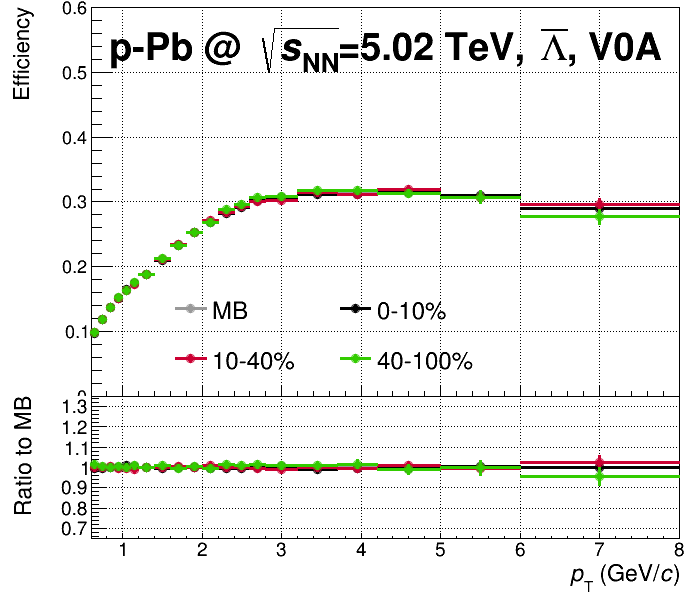
\includegraphics[width=.32\textwidth]{c02/cAntiLa_Efficiency}
%%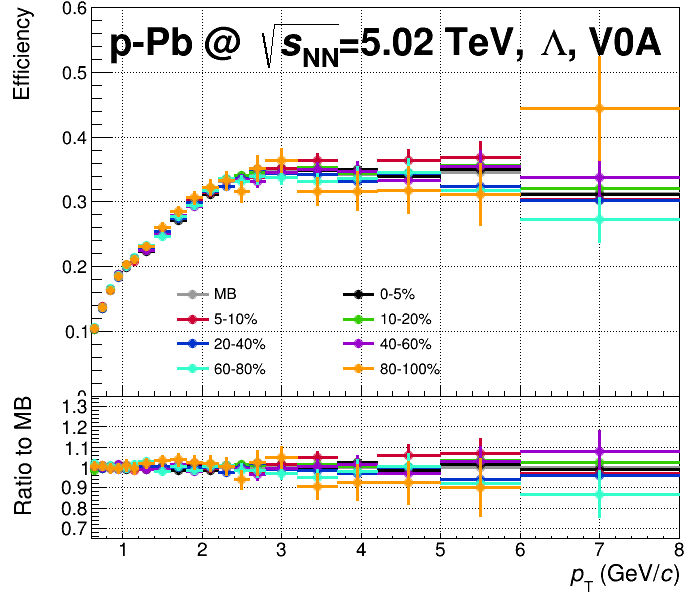
\includegraphics[width=.32\textwidth]{c02/cLambda_Efficiency}
%%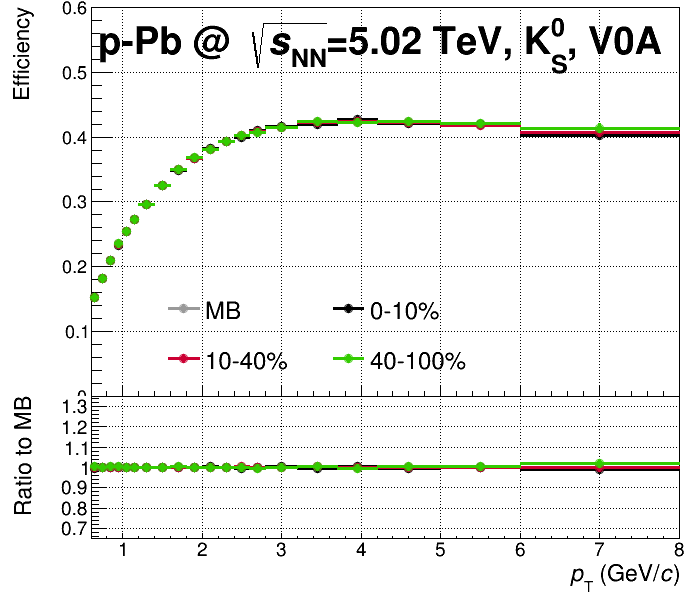
\includegraphics[width=.32\textwidth]{c02/cKshort_Efficiency}
%%\begin{center}
%%\begin{figure}[htb]
\begin{figure}[htb]
\begin{center}
%%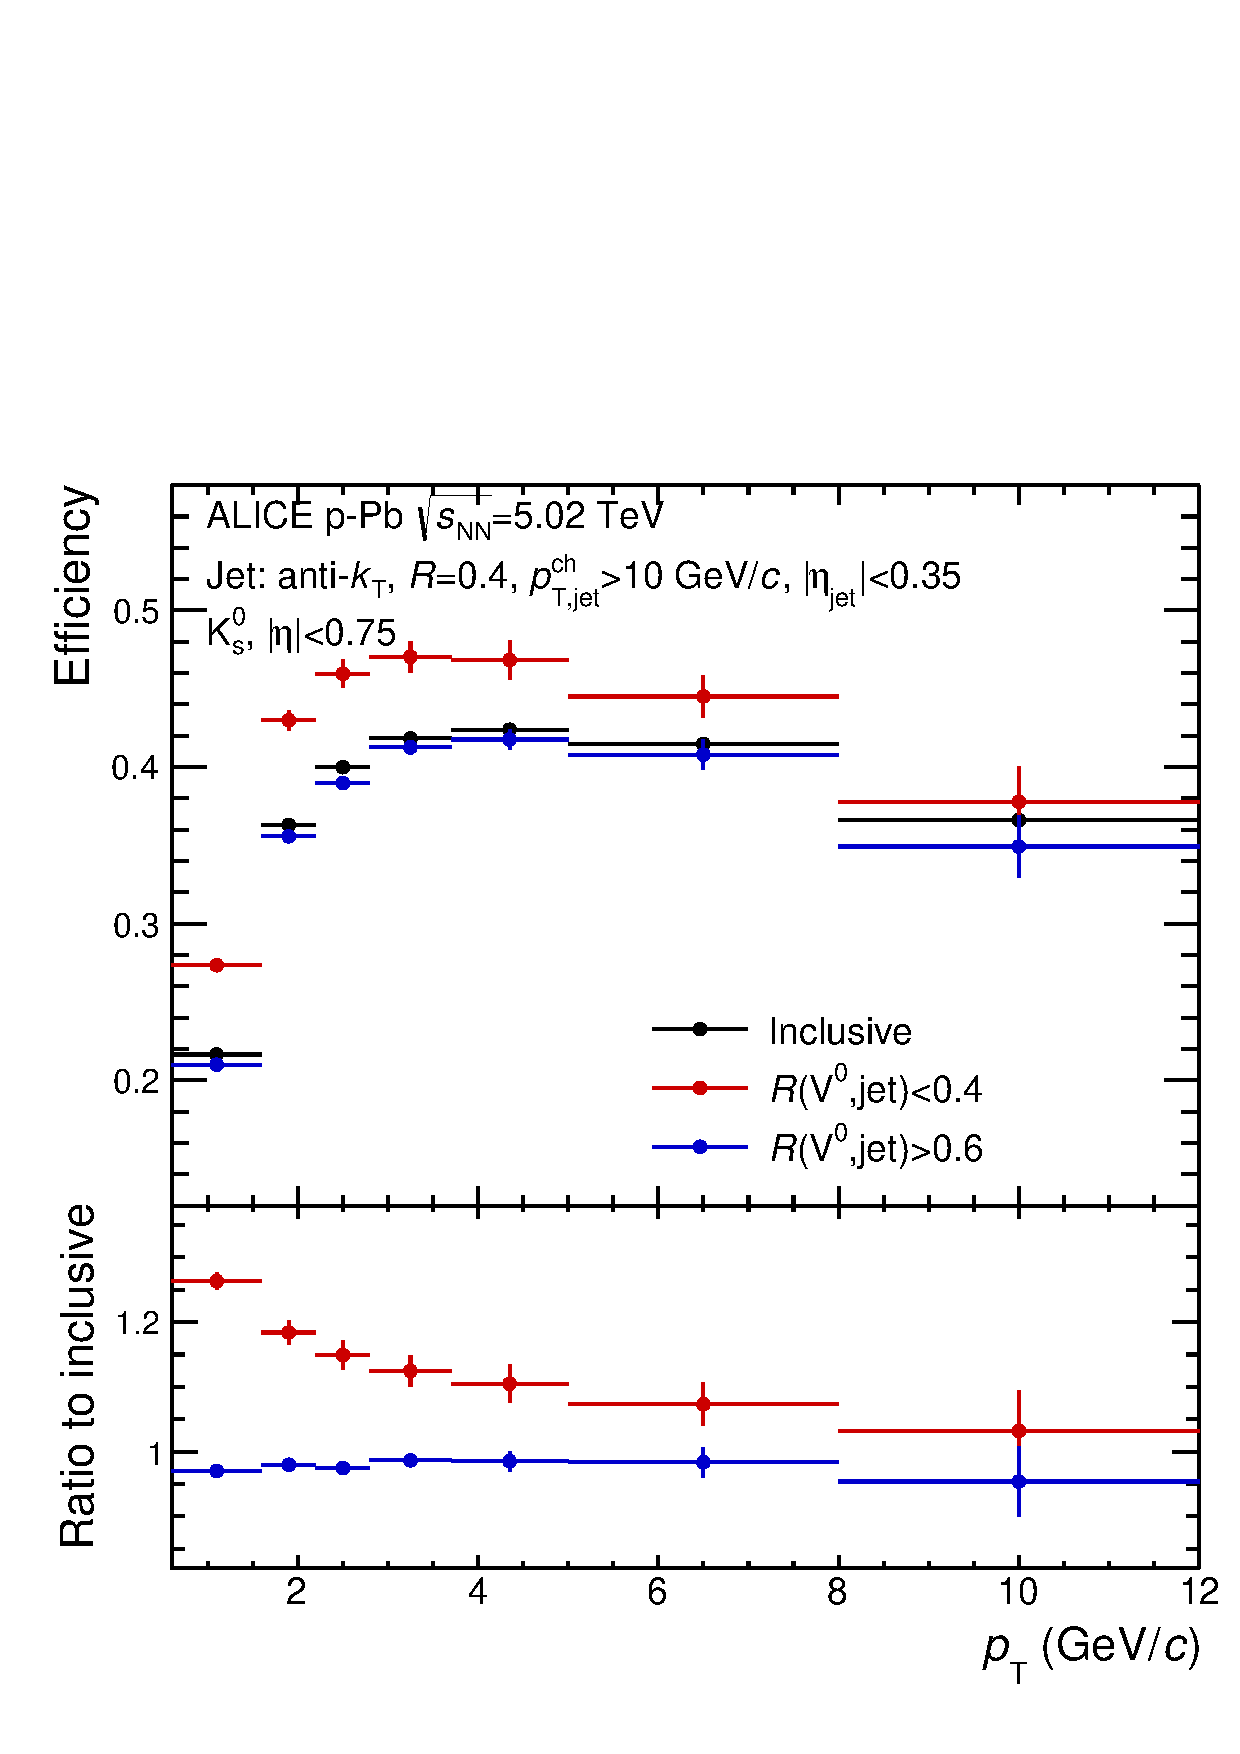
\includegraphics[width=.32\textwidth]{cEffiInJE_Kshort_JE_JR04_JC04}
%%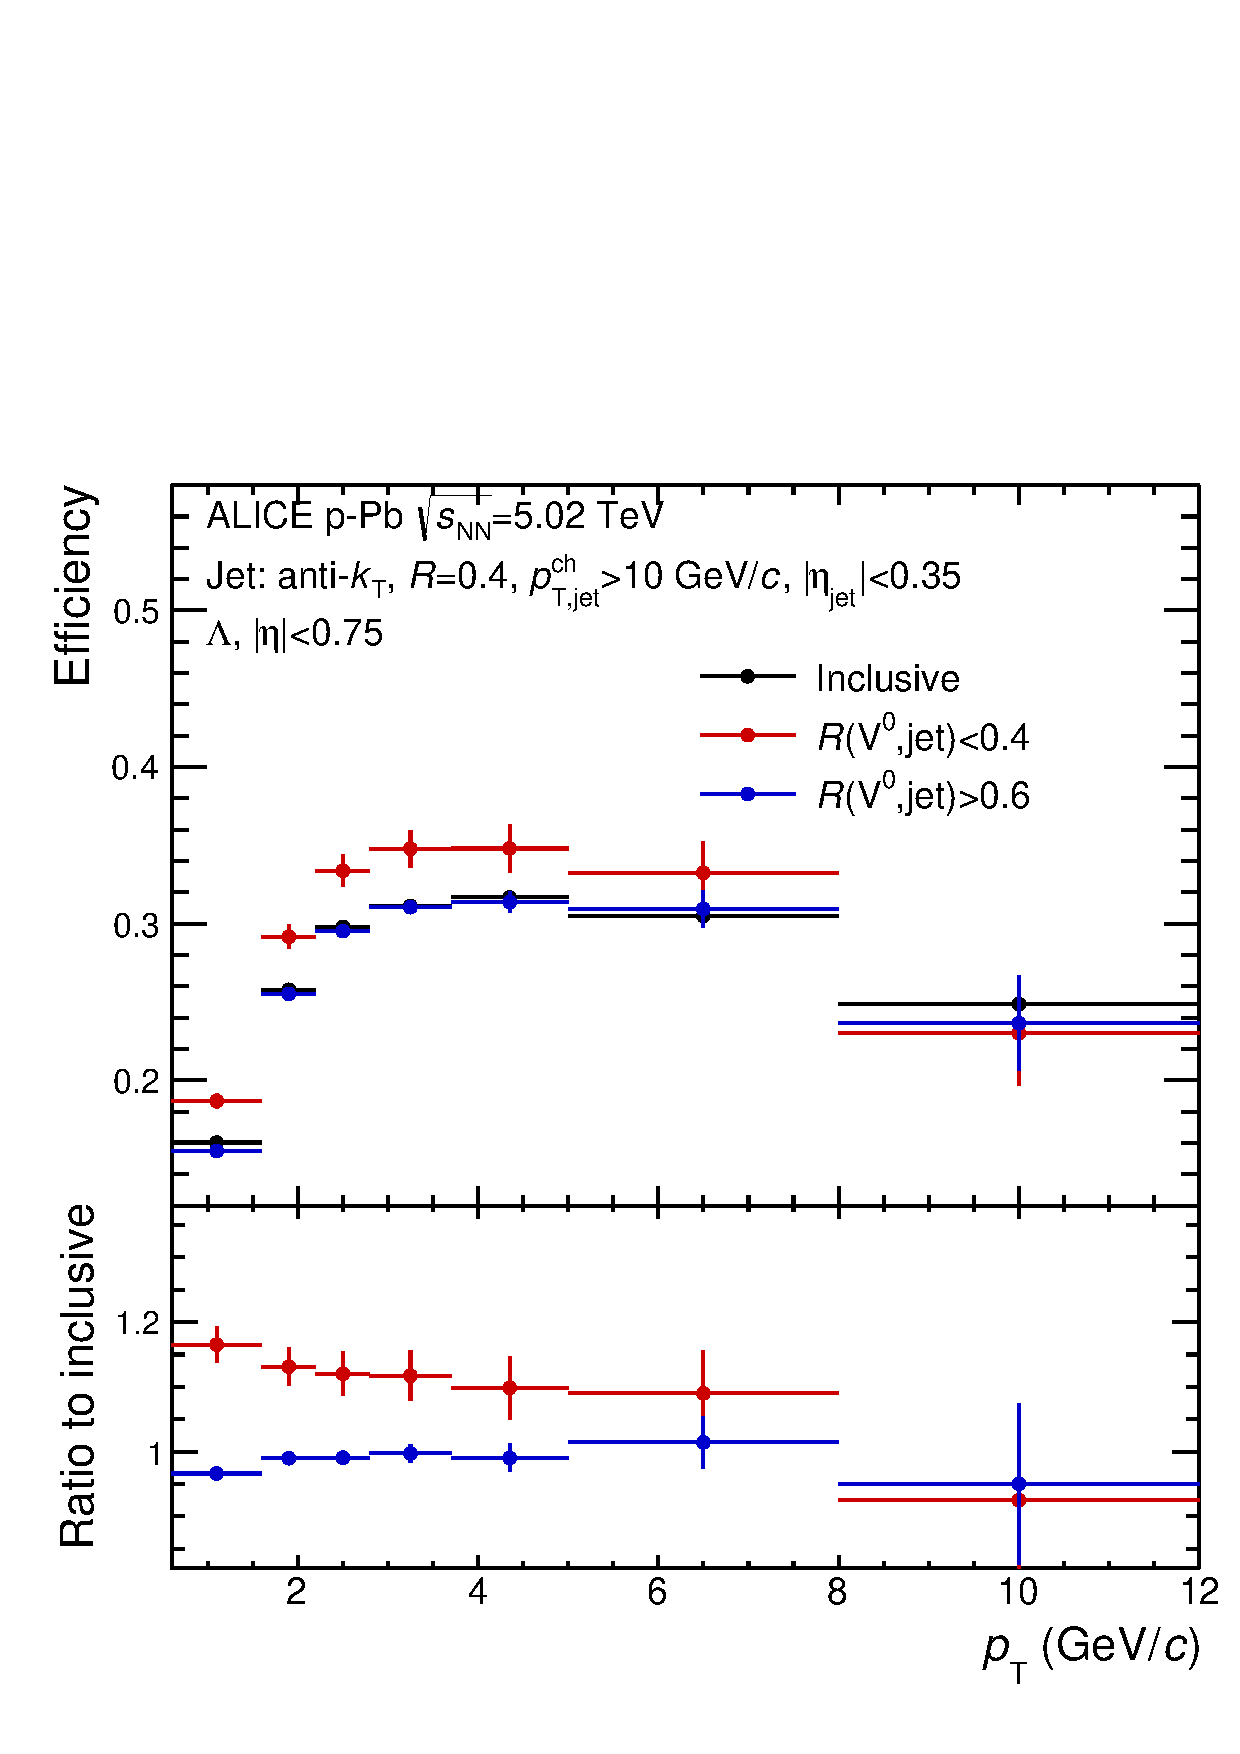
\includegraphics[width=.32\textwidth]{cEffiInJE_Lambda_JE_JR04_JC04}
%%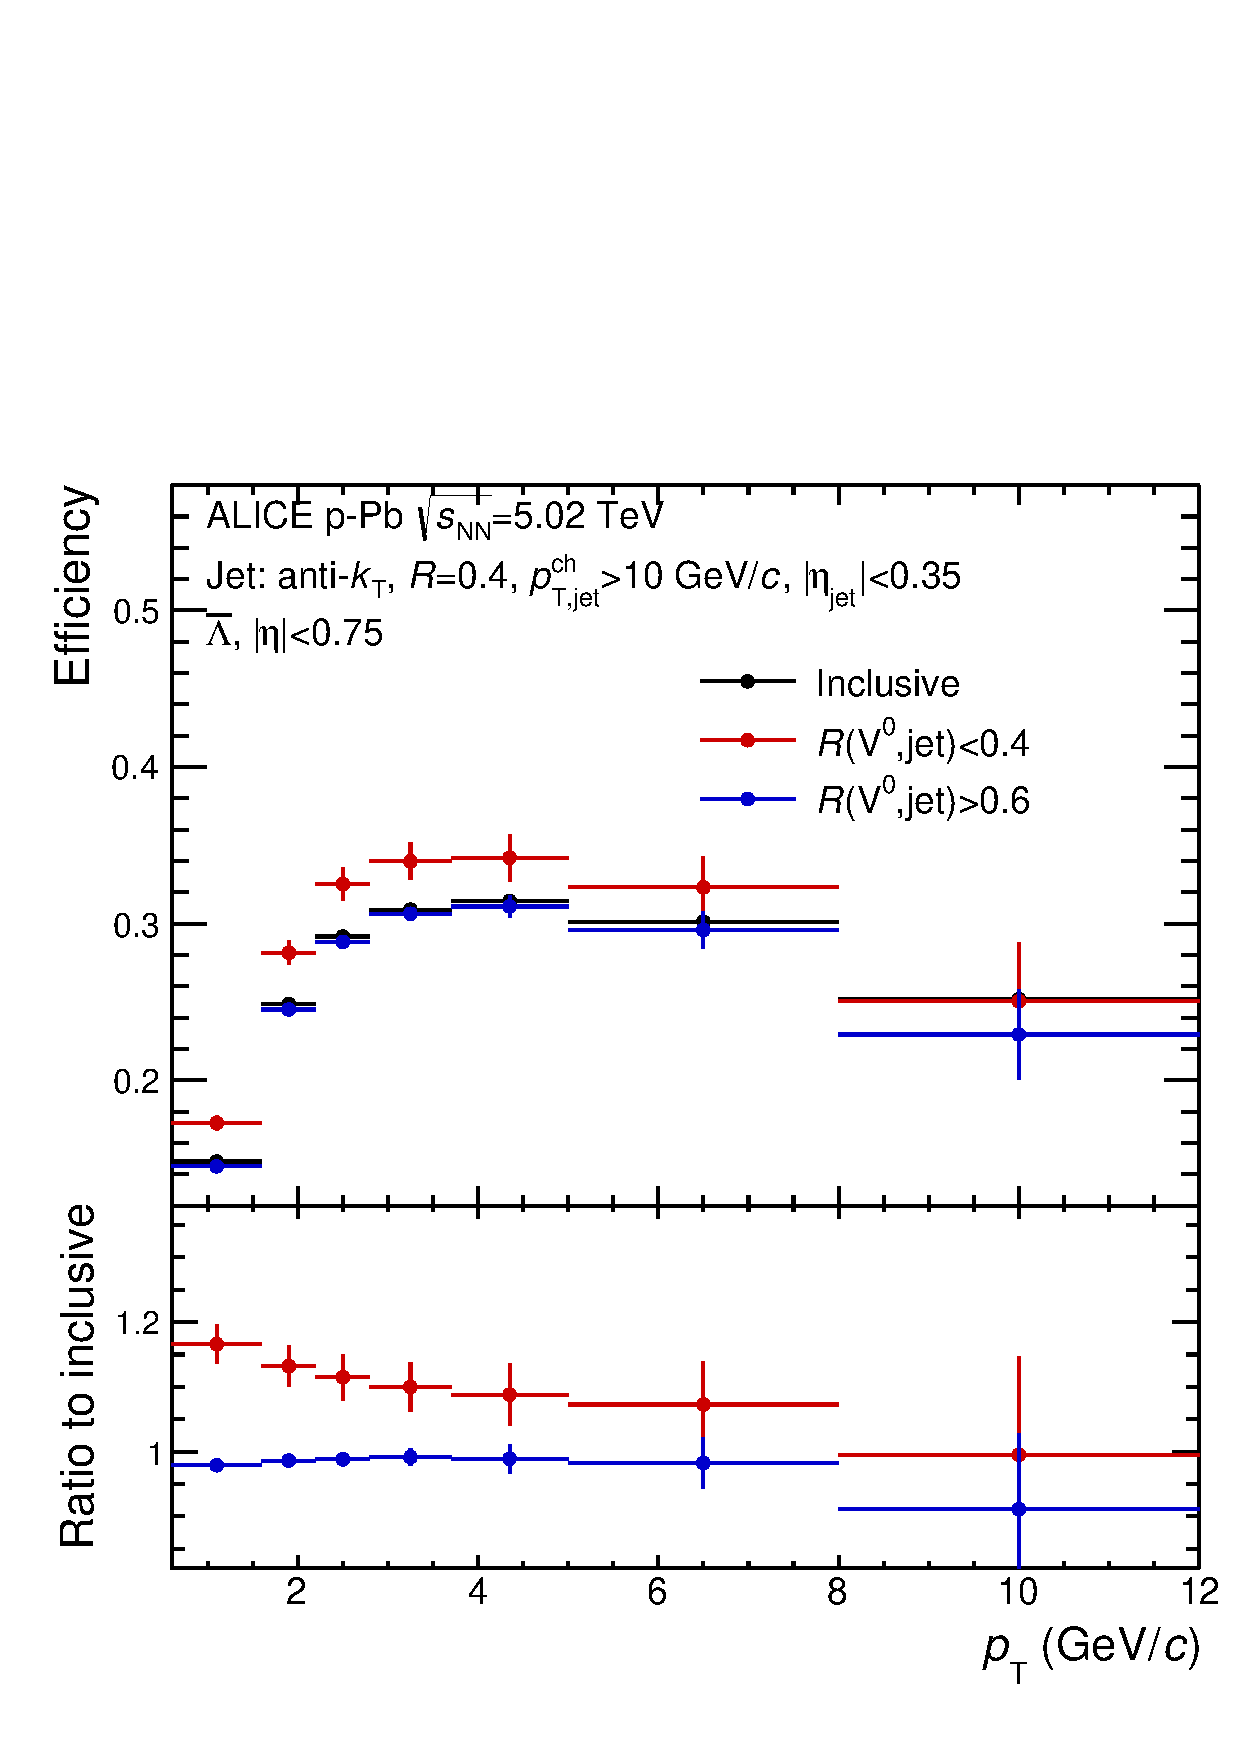
\includegraphics[width=.32\textwidth]{cEffiInJE_AntiLa_JE_JR04_JC04}
%%\includegraphics[width=.49\textwidth]{cEffiInJE_Kshort_JE_J~R04_JC04}
%%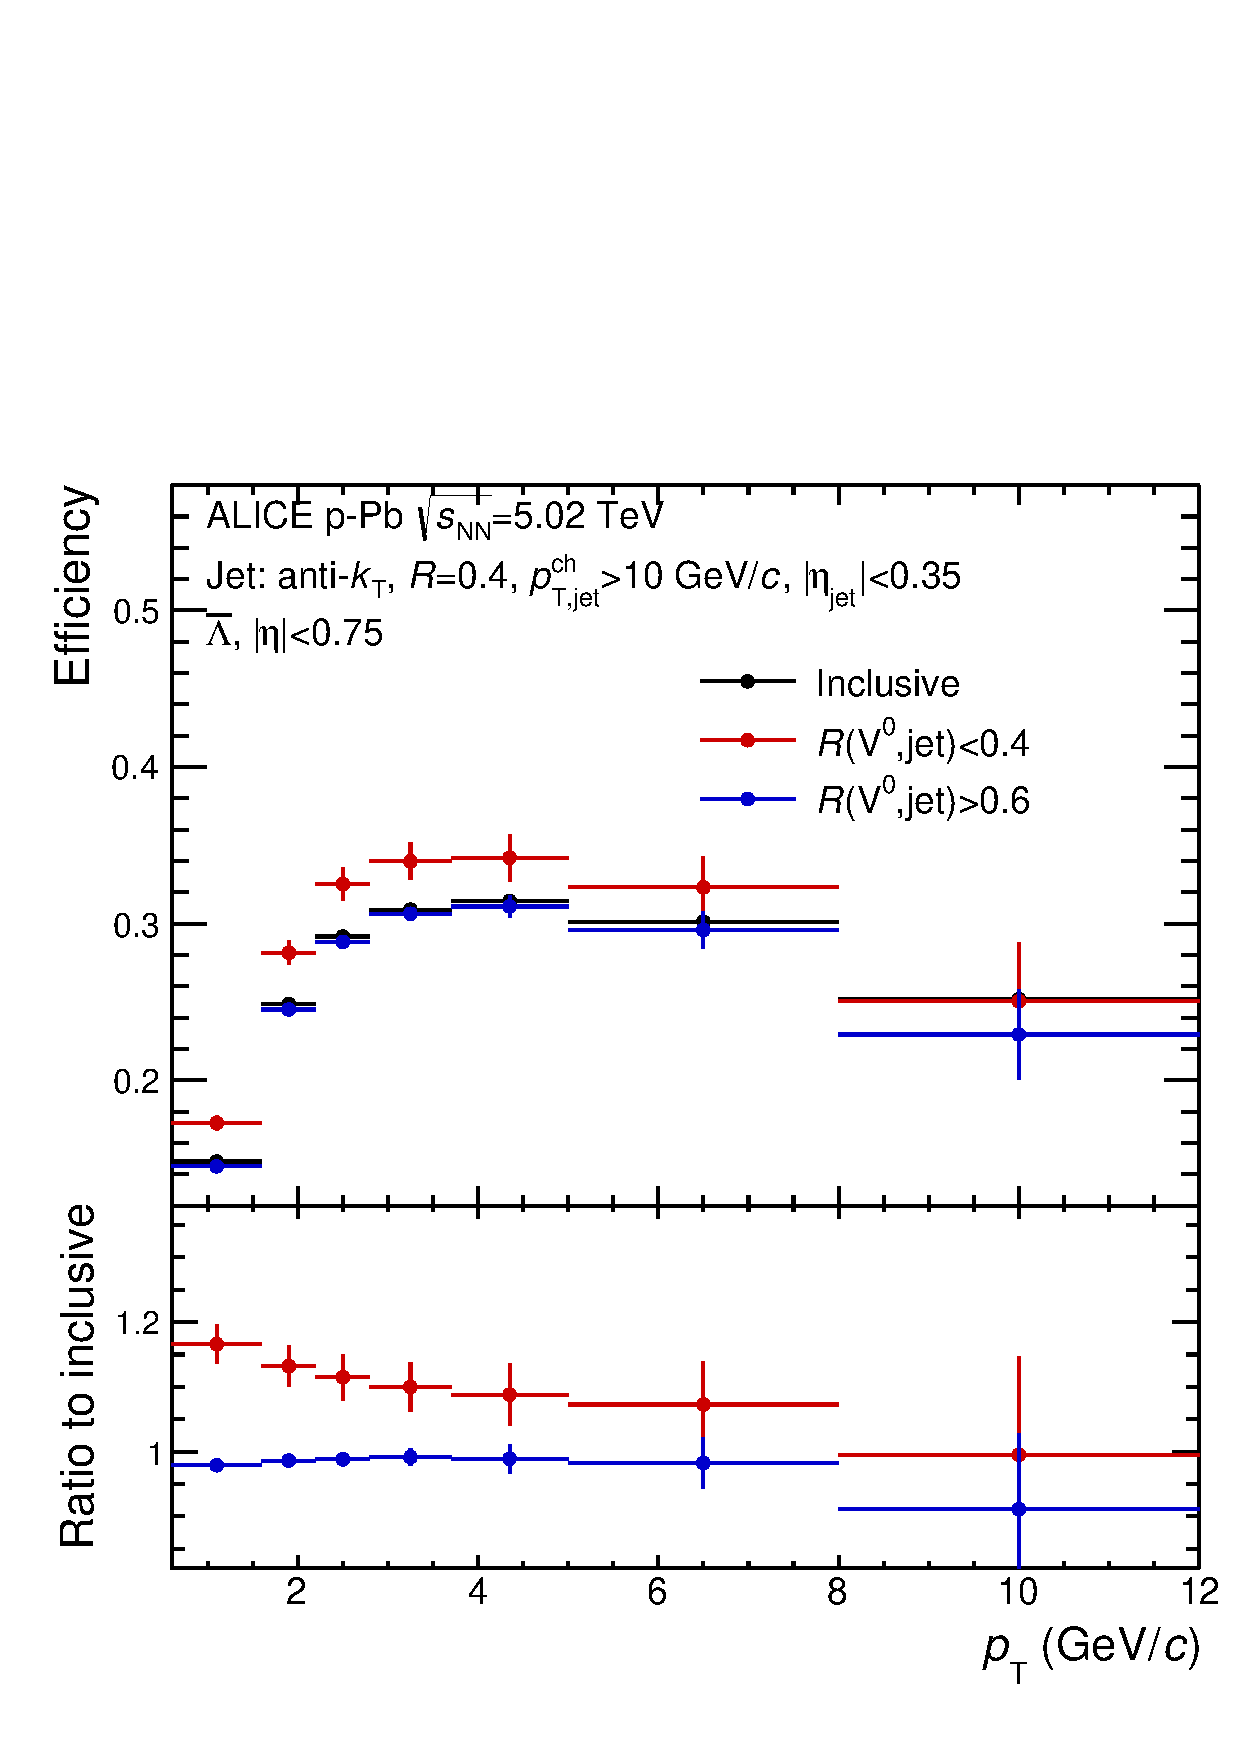
\includegraphics[width=.49\textwidth]{cEffiInJE_AntiLa_JE_JR04_JC04}
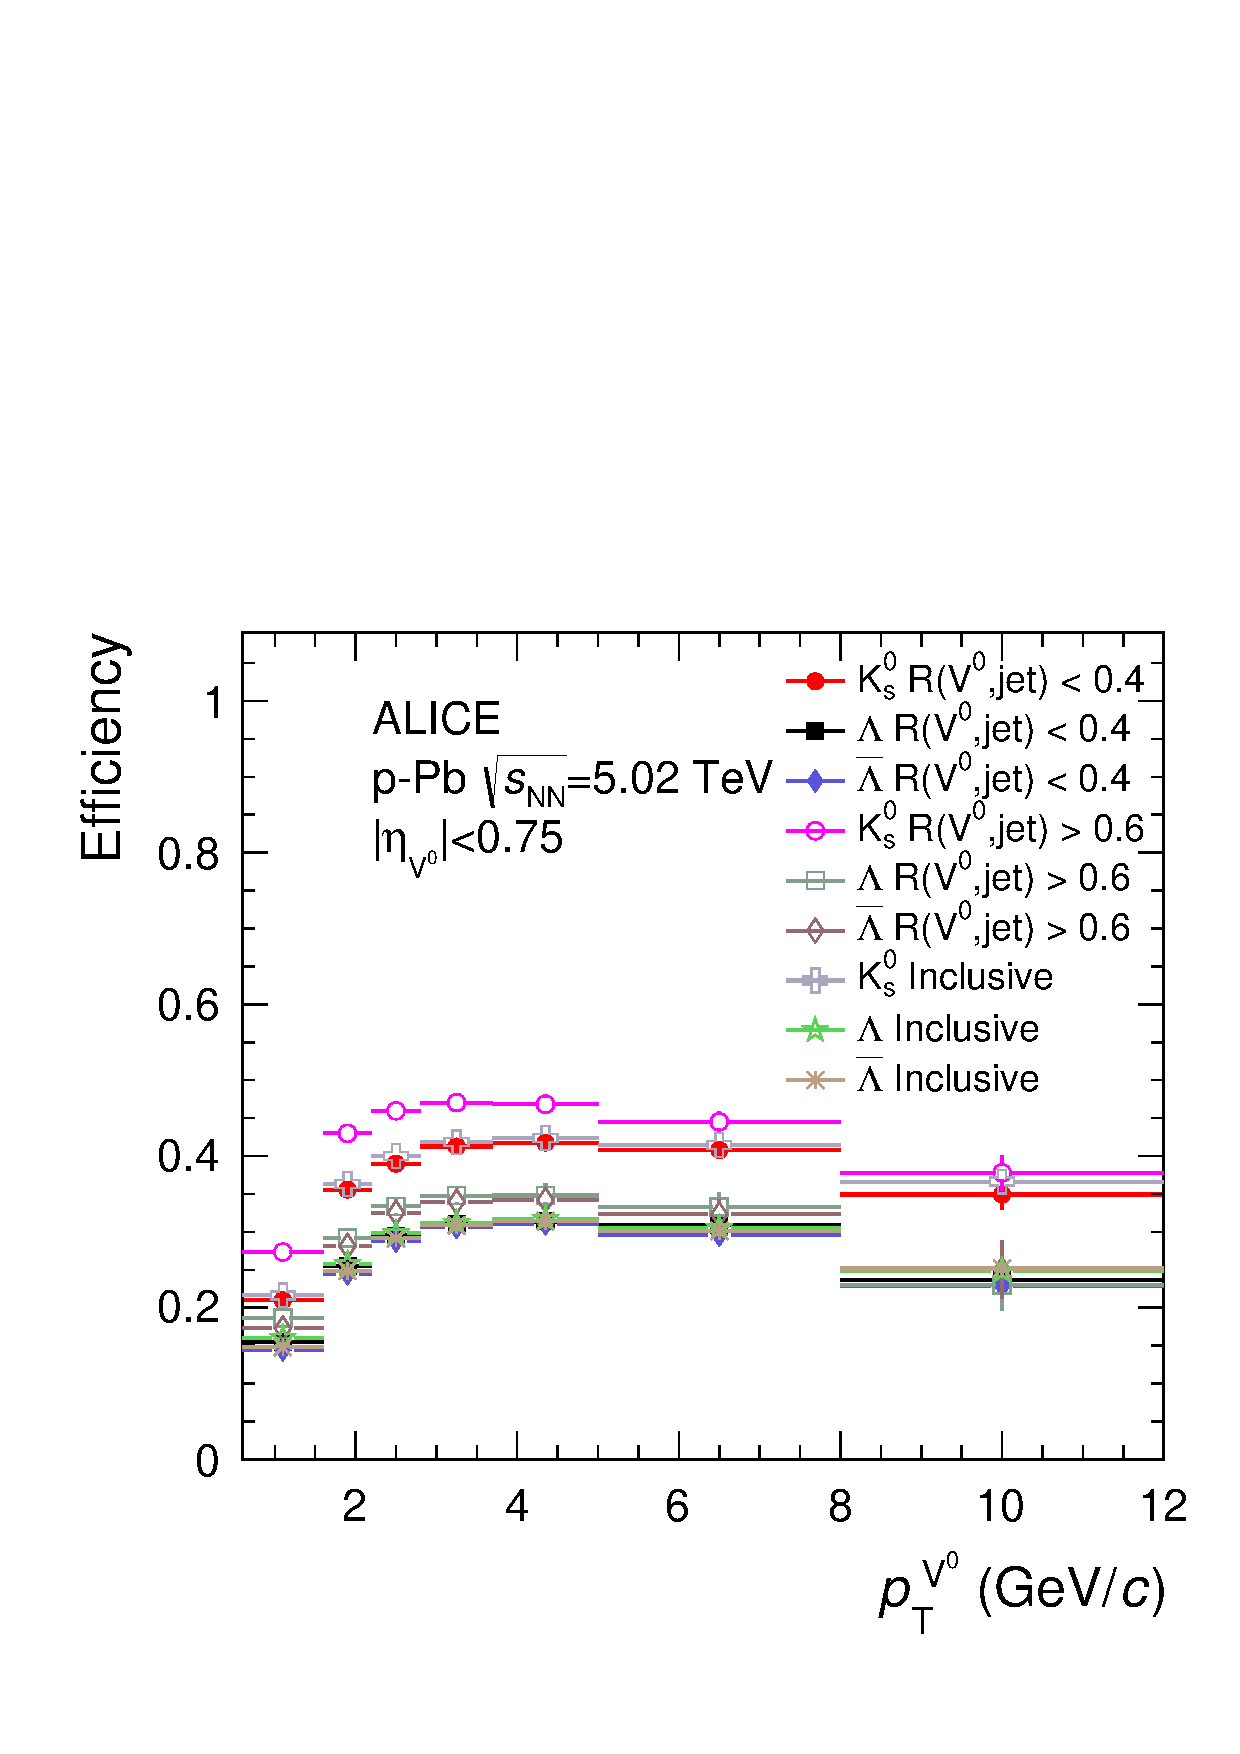
\includegraphics[width=.49\textwidth]{V__0__efficiency.pdf}
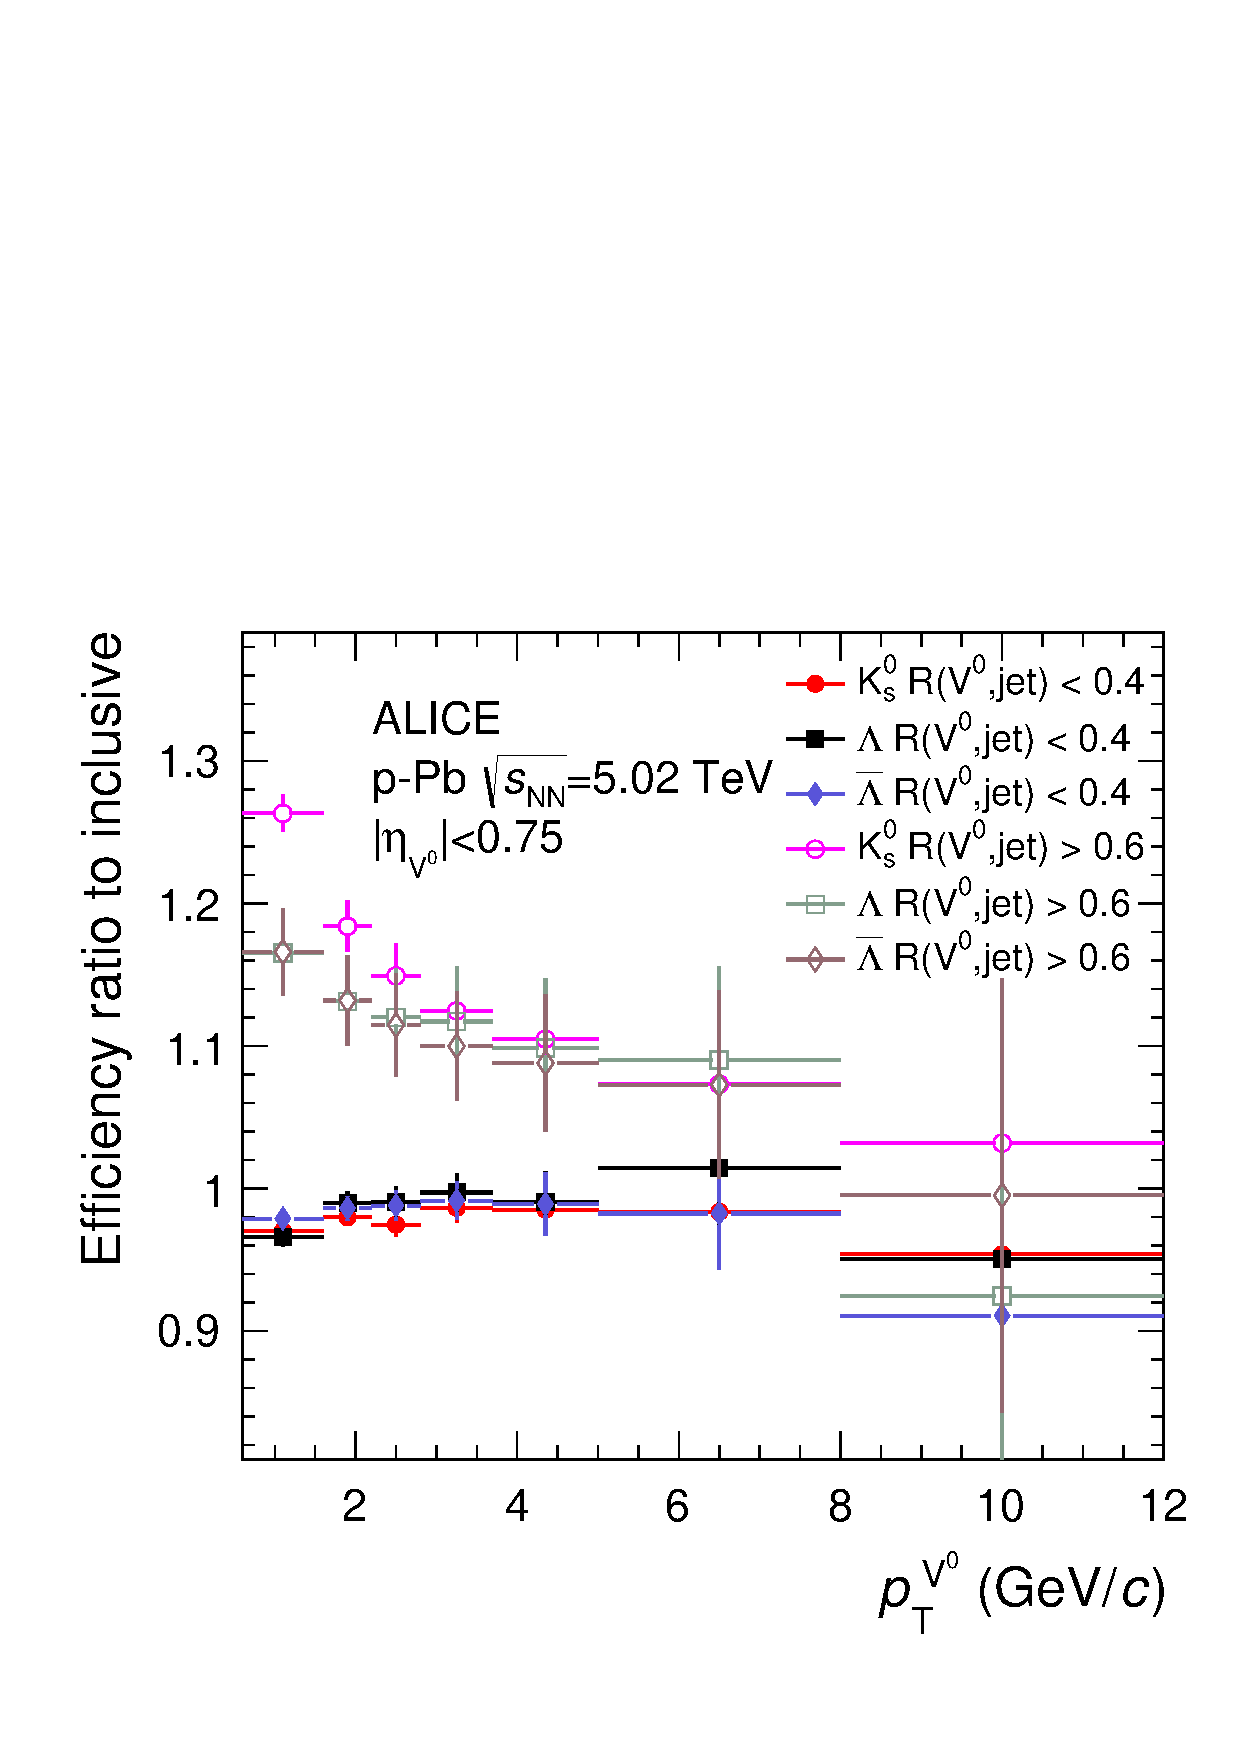
\includegraphics[width=.49\textwidth]{V__0__efficiency_ratio_to_inclusive.pdf}
\caption{Efficiency of \Vzero\ particles in \pPb\ collisions at \sqrtsnn{5.02} for three selections: inclusive, within $R_{\Vzero-{\rm jet}} <0.4$ and $R_{\Vzero-{\rm jet}} >0.6$. The efficiencies for \lda\ is consistent with the efficiency for \alda\ within about 5\% and showing similar \pt\ dependence.}
\label{fig:c02EffiIncV0s}
\end{center}
\end{figure}
Due to differences in the experimental acceptance for \Vzero\ particles associated to jets (JC) and those extracted through the various estimators of the underlying event (OC, PC, NJ) the efficiencies of \Vzero\ particles were estimated separately for every case. Figure \ref{fig:c02EffiIncV0s} shows the inclusive reconstruction efficiency for $\Vzero$ particles and the efficiency in the events containing a jet for two selections of distance $R$ from the main jet axis. In particular, for $\rvzerojet<0.4$ the efficiency at $\pt<2~\gevc$ is about 20\% greater than in the inclusive case while it approaches the inclusive case at higher \pt. The efficiency for events containing a jet varies moderately with $R$ (within a 5\%) and for every selection of $R$ the efficiencies were evaluated separately.
%%\ask{Jana: add info how does the efficiency varies with R... MP: check numbers and perhaps be more specific.} \ask{MP: added a sentence about the ratio.}

%%%%%%%%%%%%%%%%%%%%%%%%%%%%%%%%%%%%%%%%%%%%%%%%%%%%%%%%%%%%%%%%%%
%%\subsection{Feed-down subtraction for \lda\ and \alda}

The \pt\ differential yields of \lda\ and \alda\ reconstructed for each selection (JC and UE selections) were in addition also corrected for the feed-down from $\Xi$ decays.
%%The correction was applied before the efficiency corrections.
The $\Xi$ production in jets (JC) was estimated based on measurements of the multi-strange baryons and their decays at high-\pt\ performed in \pPb\ collisions \cite{Adam:2015vsf} and extrapolated to the lower \pt\ using PYTHIA event generator and full detector simulations.
The applied correction amounts to 15\% and is independent of the \lda\ and \alda\ momentum.
%%\ask{MP: check numbers}
Conversely, \lda\ yields were not corrected for the feed-down from $\Omega^{-}$ baryons nor for the feed-down from non-weak decays of $\Sigma^{0}$ and $\Sigma^{*}(1385)$ family as these contributions are neglibible as compared to the systematic uncertainties of the present measurement.

%%%%%%%%%%%%%%%%%%%%%%%%%%%%%%%%%%%%%%%%%%%%%%%%%%%%%%%%%%%%%%%%%%

\subsection{Systematic uncertainties}
\label{sec:uncertainties}
%%\subsection{Uncertainties in \Vzero\ particle reconstruction}
%% \ask{MP: remove the table; adjust the figure (remove fluctuations) and add the proper text.}
The main sources in the \Vzero\ particle reconstruction are the level of knowledge of the detector material (resulting in a 4\% uncertainty), the track selection (up to 4\%), the feed-down correction for the \lda\ (5\% for $\pt<3.7~\gevc$ and 7\% for $\pt>3.7~\gevc$), the proper lifetime selection criteria (up to 3\%) and the topological selections that contribute up to 1.5\% depending on transverse momentum and particle species.
%%\ask{explain ``competing \vzero's '' and ``proper lifetime''}
%%The uncertainties are summarized in Table \ref{tab:v0syst}. Figure \ref{fig:systUncert} presents the \pt\ dependence of these uncertainties with the exception of the uncertainty related to the detector material that is \pt\ independent.

The $\pT$-dependent uncertainties on the extracted yields of \Vzero\ particles are shown in Fig. \ref{fig:systUncert} for \ks\ mesons and \alda\ baryons.
To calculate the total uncertainty on the yields the individual uncertainties on track selection, material budged, feed-down corrections and the listed \Vzero\ selections are added in quadrature.

{\bf Particle identification (PID).} Uncertainty due to the particle identification cuts was estimated by varying the cuts on the $\dedx$ in the TPC from a default $5 \sigma$ to 4, 6 and 7 standard deviations from the nominal $\dedx$ for pions and protons.
%% The uncertainty is highest at high \pt\ reaching $\about 1\%$ for $\pt > 5 \gevc$ kaons and $\about 2\%$ for $\pt > 8 \gevc$ \lda and \alda.

{\bf Track selection.} Uncertainty on the \Vzero\ yields originating from the track selection was estimated by repeating the analysis with the increased number of required TPC space points per track by about 7\% and 15\% from the nominal requirement of 70 points.
%% \ask{MP: it is very difficult to find in ALICE papers this type of definition... ;-(}

{\bf Topological selection.} The uncertainty associated to topological cuts on the \Vzero\ candidates (the two dimensional decay radius, daughter track DCA to primary vertex, minimum DCA of \Vzero\ daughters, and maximum cosine of the pointing angle) was obtained by varying the parameters of the selections for each of the \Vzero\ species separately as described in detail in \cite{Abelev:2013haa}.
%%For \ks\ the uncertainty reaches 1.5\% below 2 \gevc\ and decreased to 1\% at higher \pT. For \lda\ baryons the uncertainty reaches maximum of about 1.5\% at about 2 \gevc\ and decreases to 0.5\% at 6 \gevc\ and above.

{\bf Proper lifetime selection.} The uncertainty due to the cuts on the proper lifetime of the \Vzero\ candidates defined as the product of mass $m$, decay length $L$ and the inverse of particle's momentum $p$ ($mLc/p < 20~{\rm cm}$ for \ks\ and $mLc/p <30~{\rm cm}$ for \lda\ baryons) was obtained by redoing the analysis with different cuts (12 and 40 ${\rm cm}$ for \ks\ and 20 and 40 ${\rm cm}$ for \lda\ and \alda).
%%For \ks\ the uncertainty was found below 0.5\% below 4 \gevc\ and negligible at higher \pt. For \lda\ baruons uncertainty reached 5\% at $\pt < 2~\gevc$ falling below 1\% at $\pt > 5~\gevc$.

{\bf Competing \Vzero\ selection.} To obtain the uncertainty related to the cut on the competing \Vzero\ particles defined as the absolute mass difference between \Vzero\ candidate and the rest mass of the competing weakly decaying hadron ($m>5~\mevcc$ for \ks\ and $m>10~\mevcc$ for \lda) the analysis was repeated with 3 and 6 \mevcc\ for \ks\ and with no rejection for \lda\ baryons.
%%The uncertainty reaches of a~bout 0.5\% for \ks\ at high \pt. For \lda\ particles the uncertainty shows a peak at $\pt \sim 1.2~\gevc$ th~en decreases below 1\%, reaching 4.5\% for $\pt > 8~\gevc$

\begin{figure}[htbp]
	\centering
	%%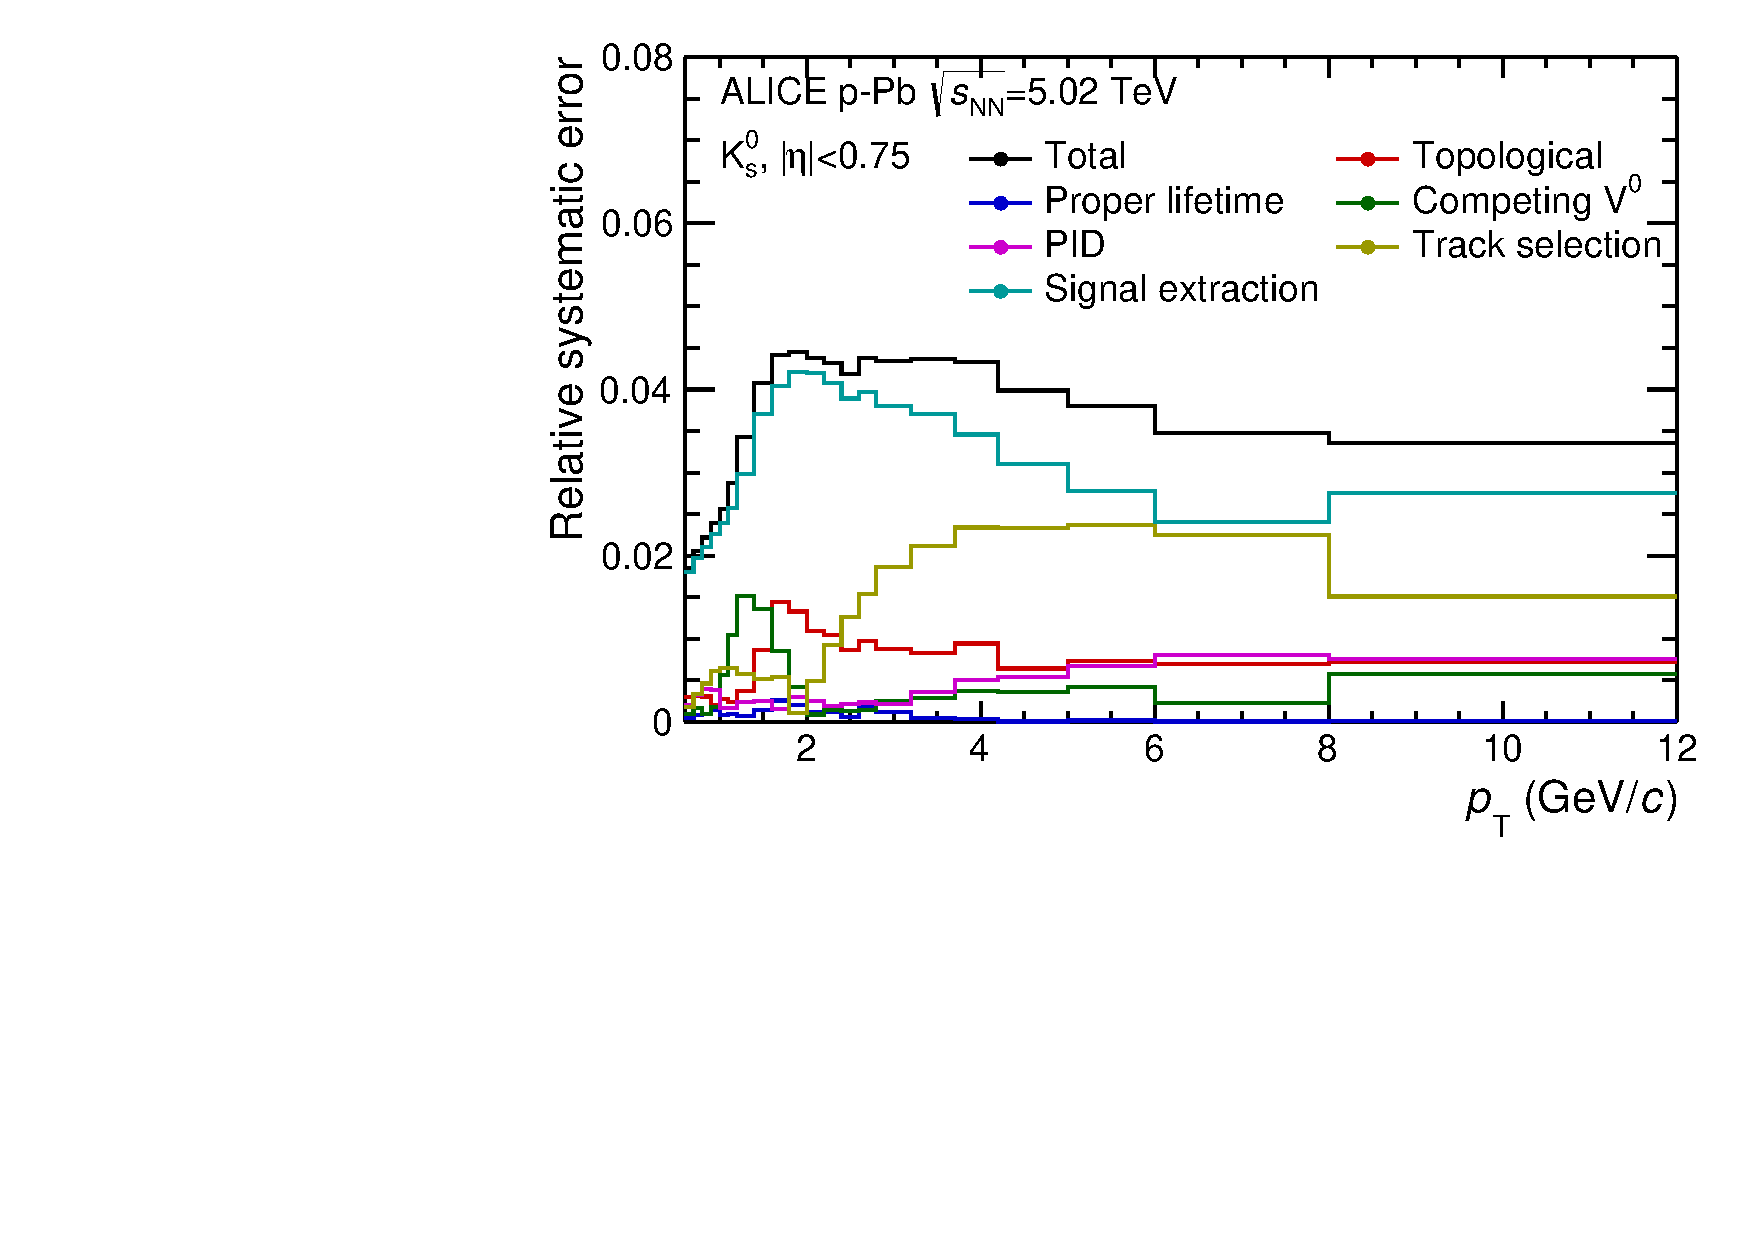
\includegraphics[width=0.32\textwidth]{cSystIncl_Kshort}
	%%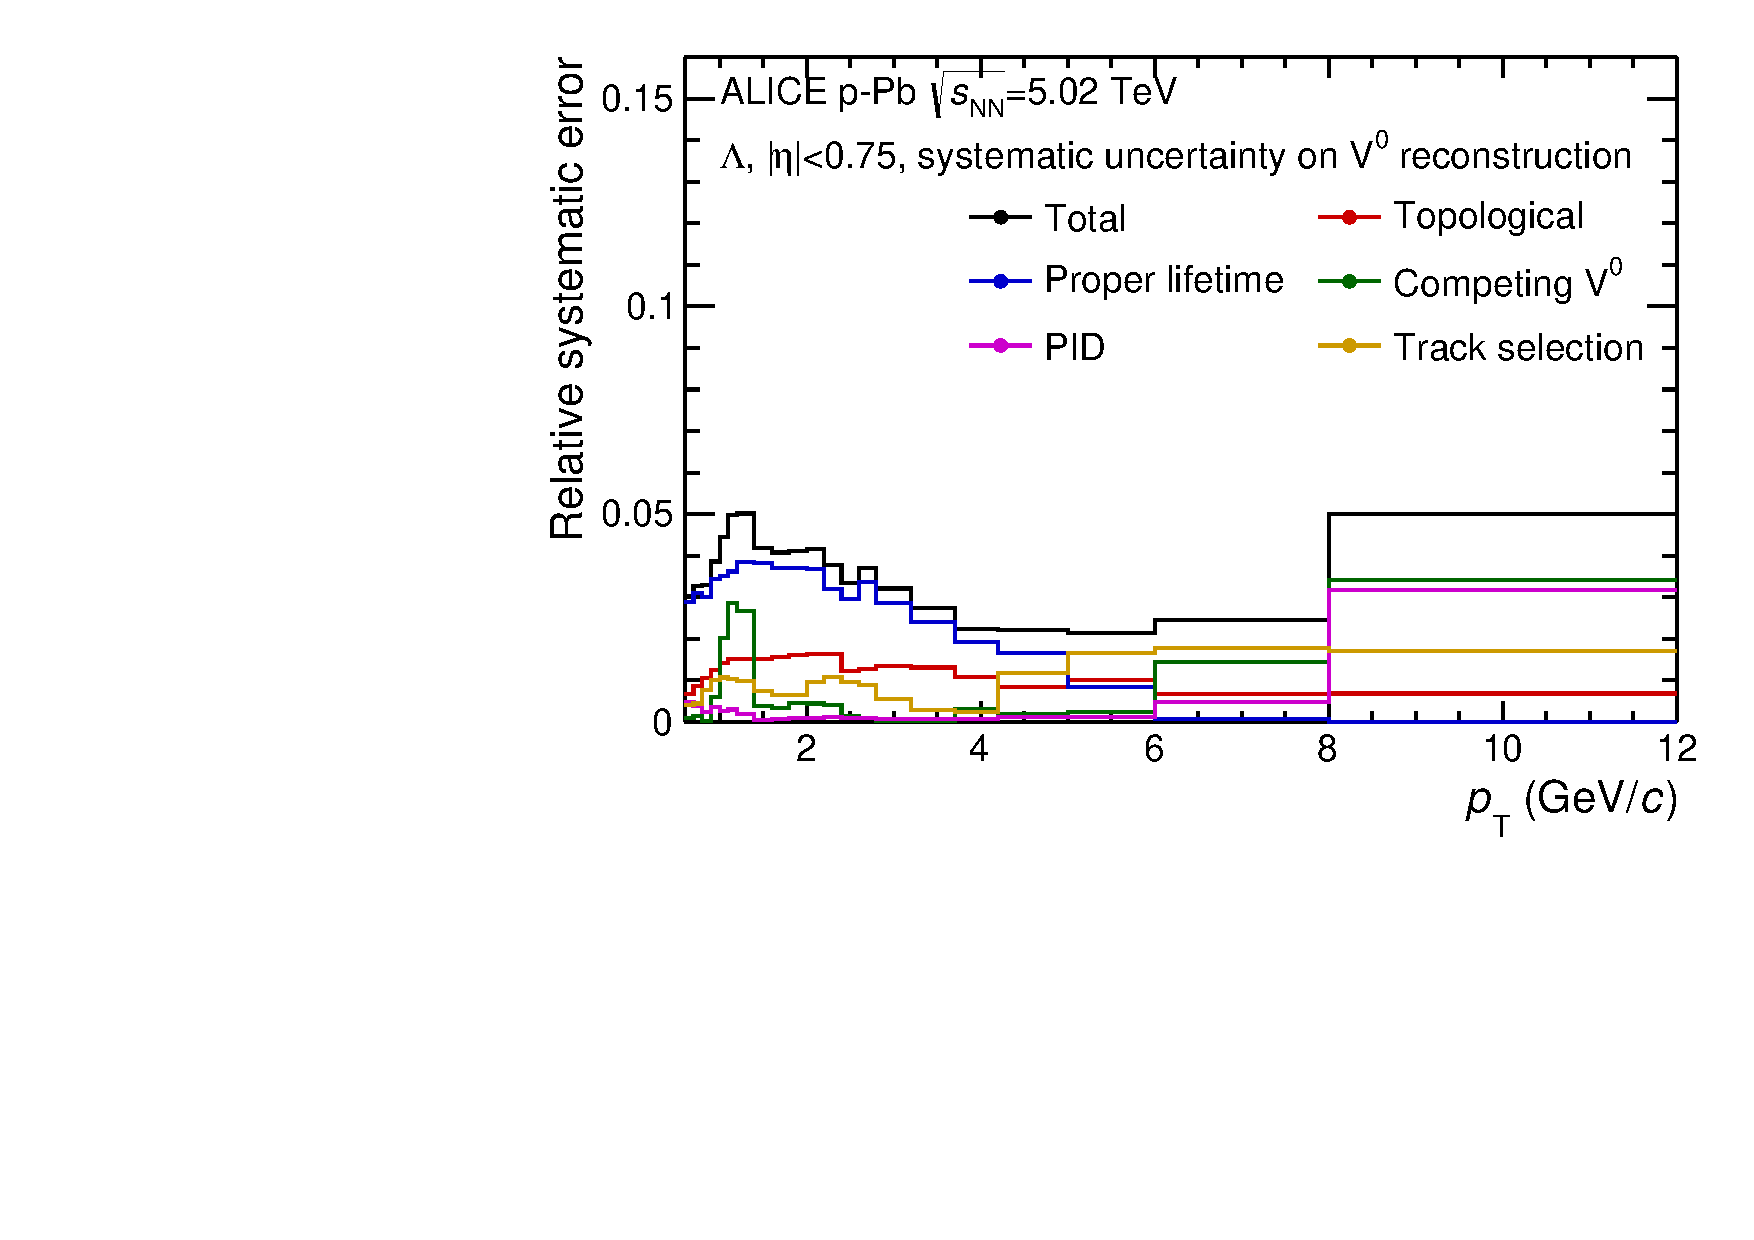
\includegraphics[width=0.32\textwidth]{cSystIncl_Lambda}
	%%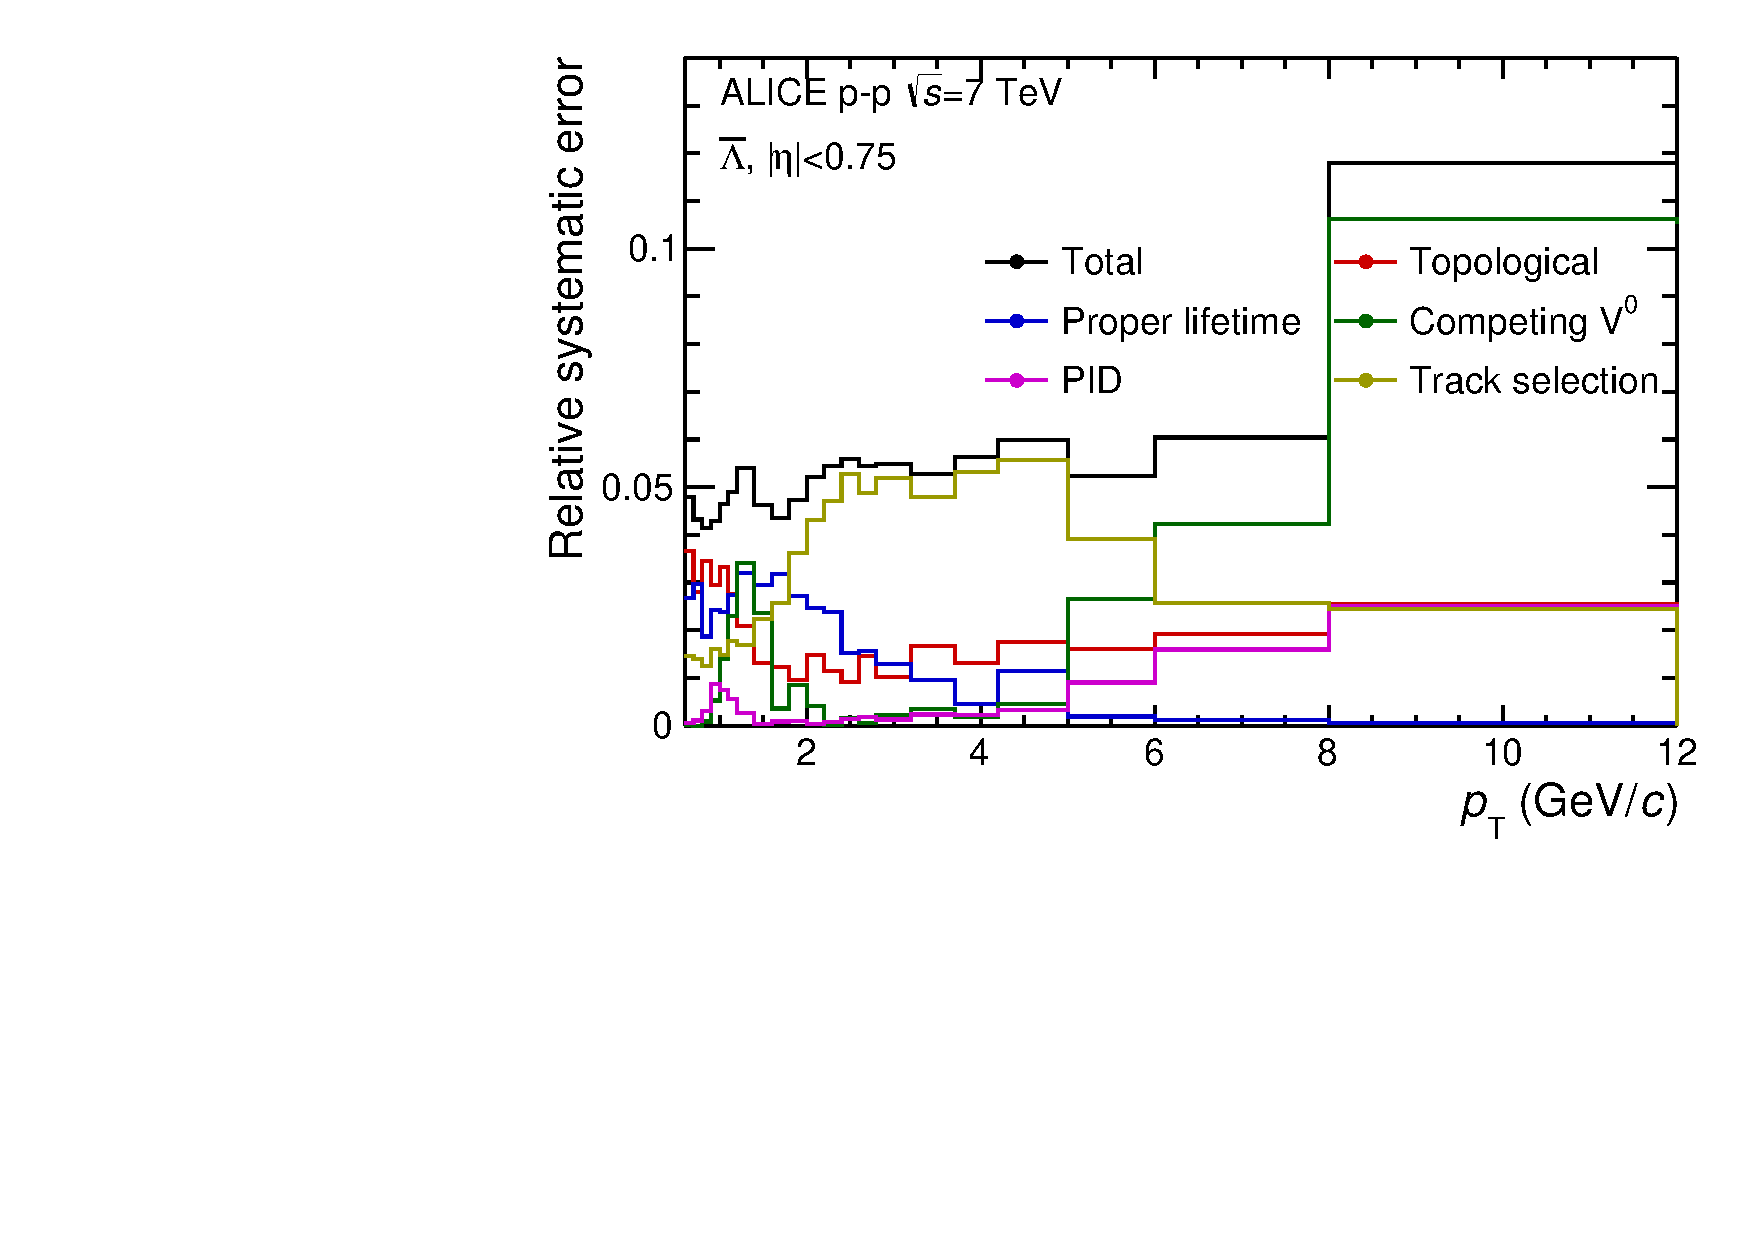
\includegraphics[width=0.32\textwidth]{cSystIncl_AntiLa}
	%%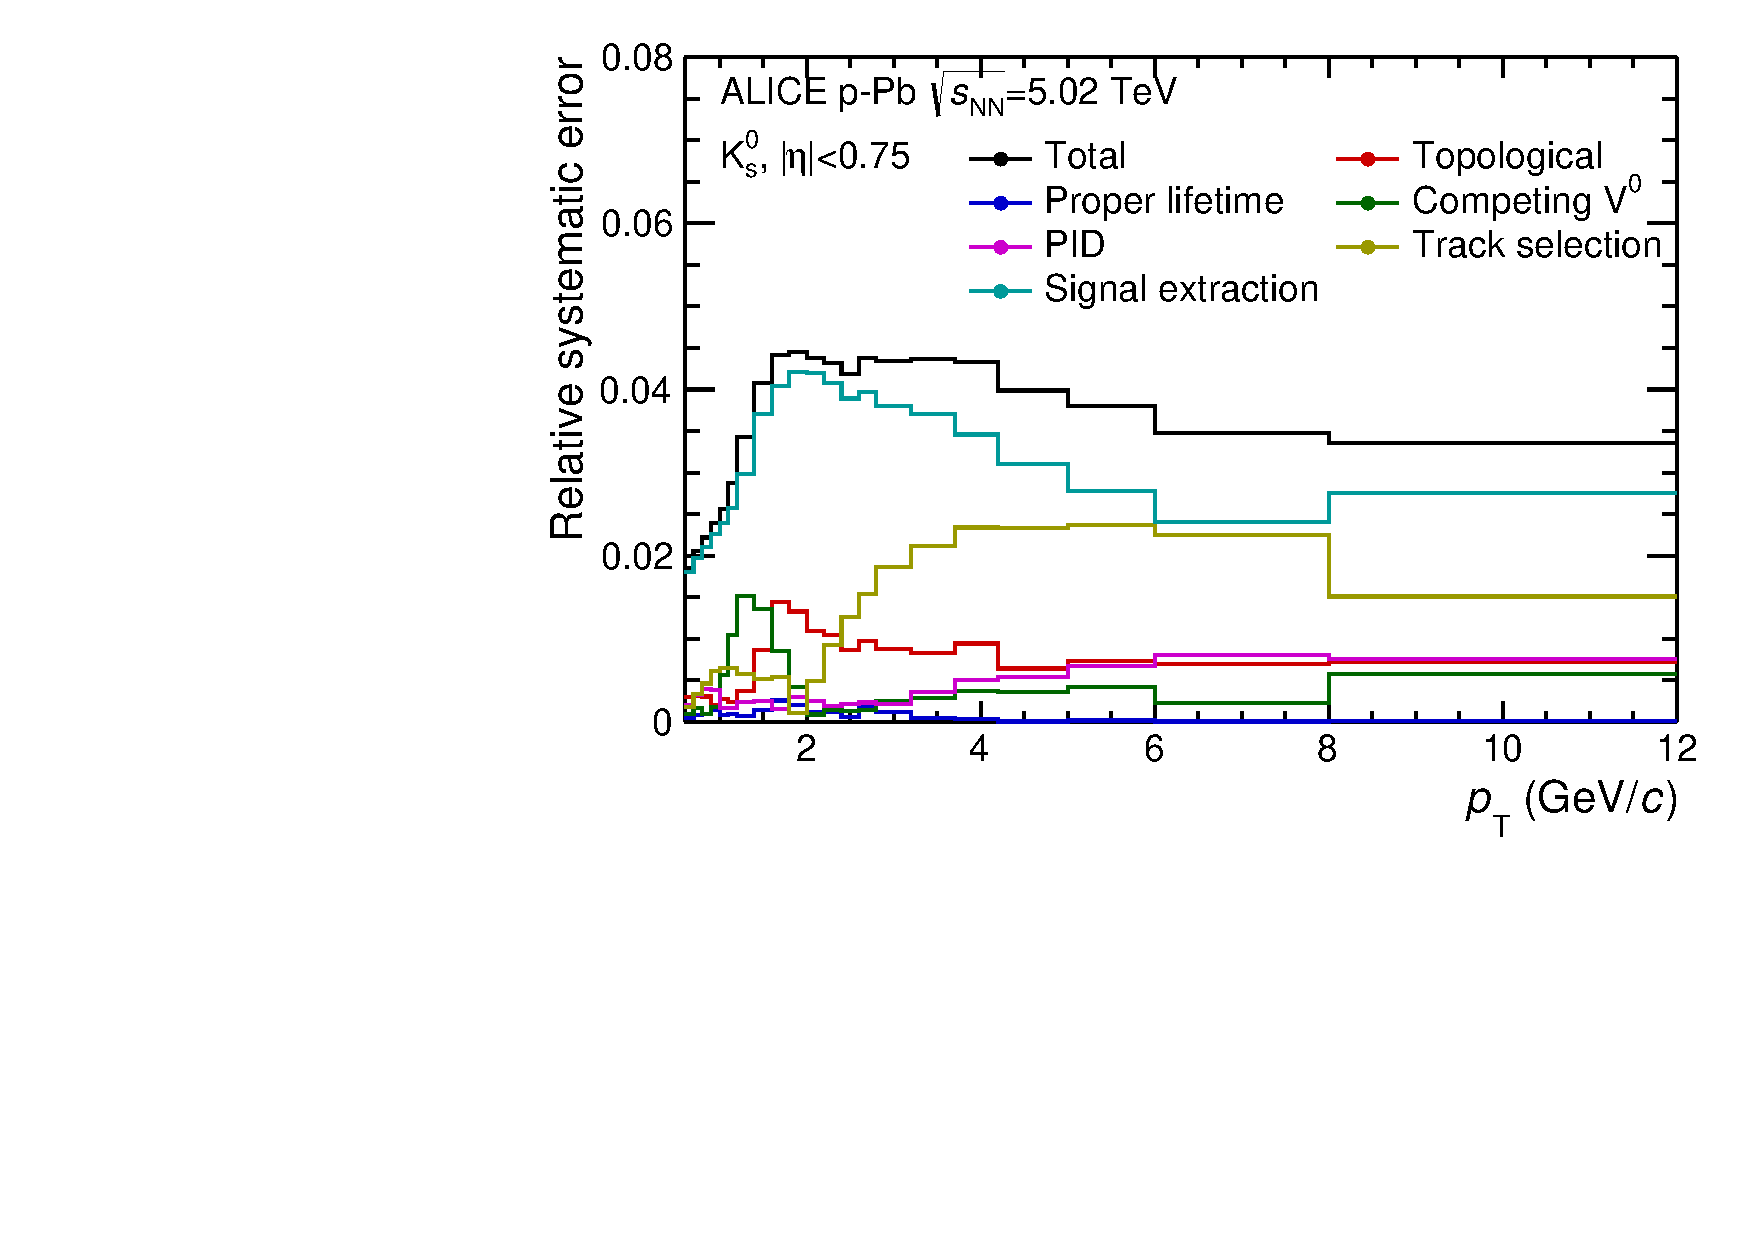
\includegraphics[width=.49\textwidth]{cSystIncl_Kshort}
	%%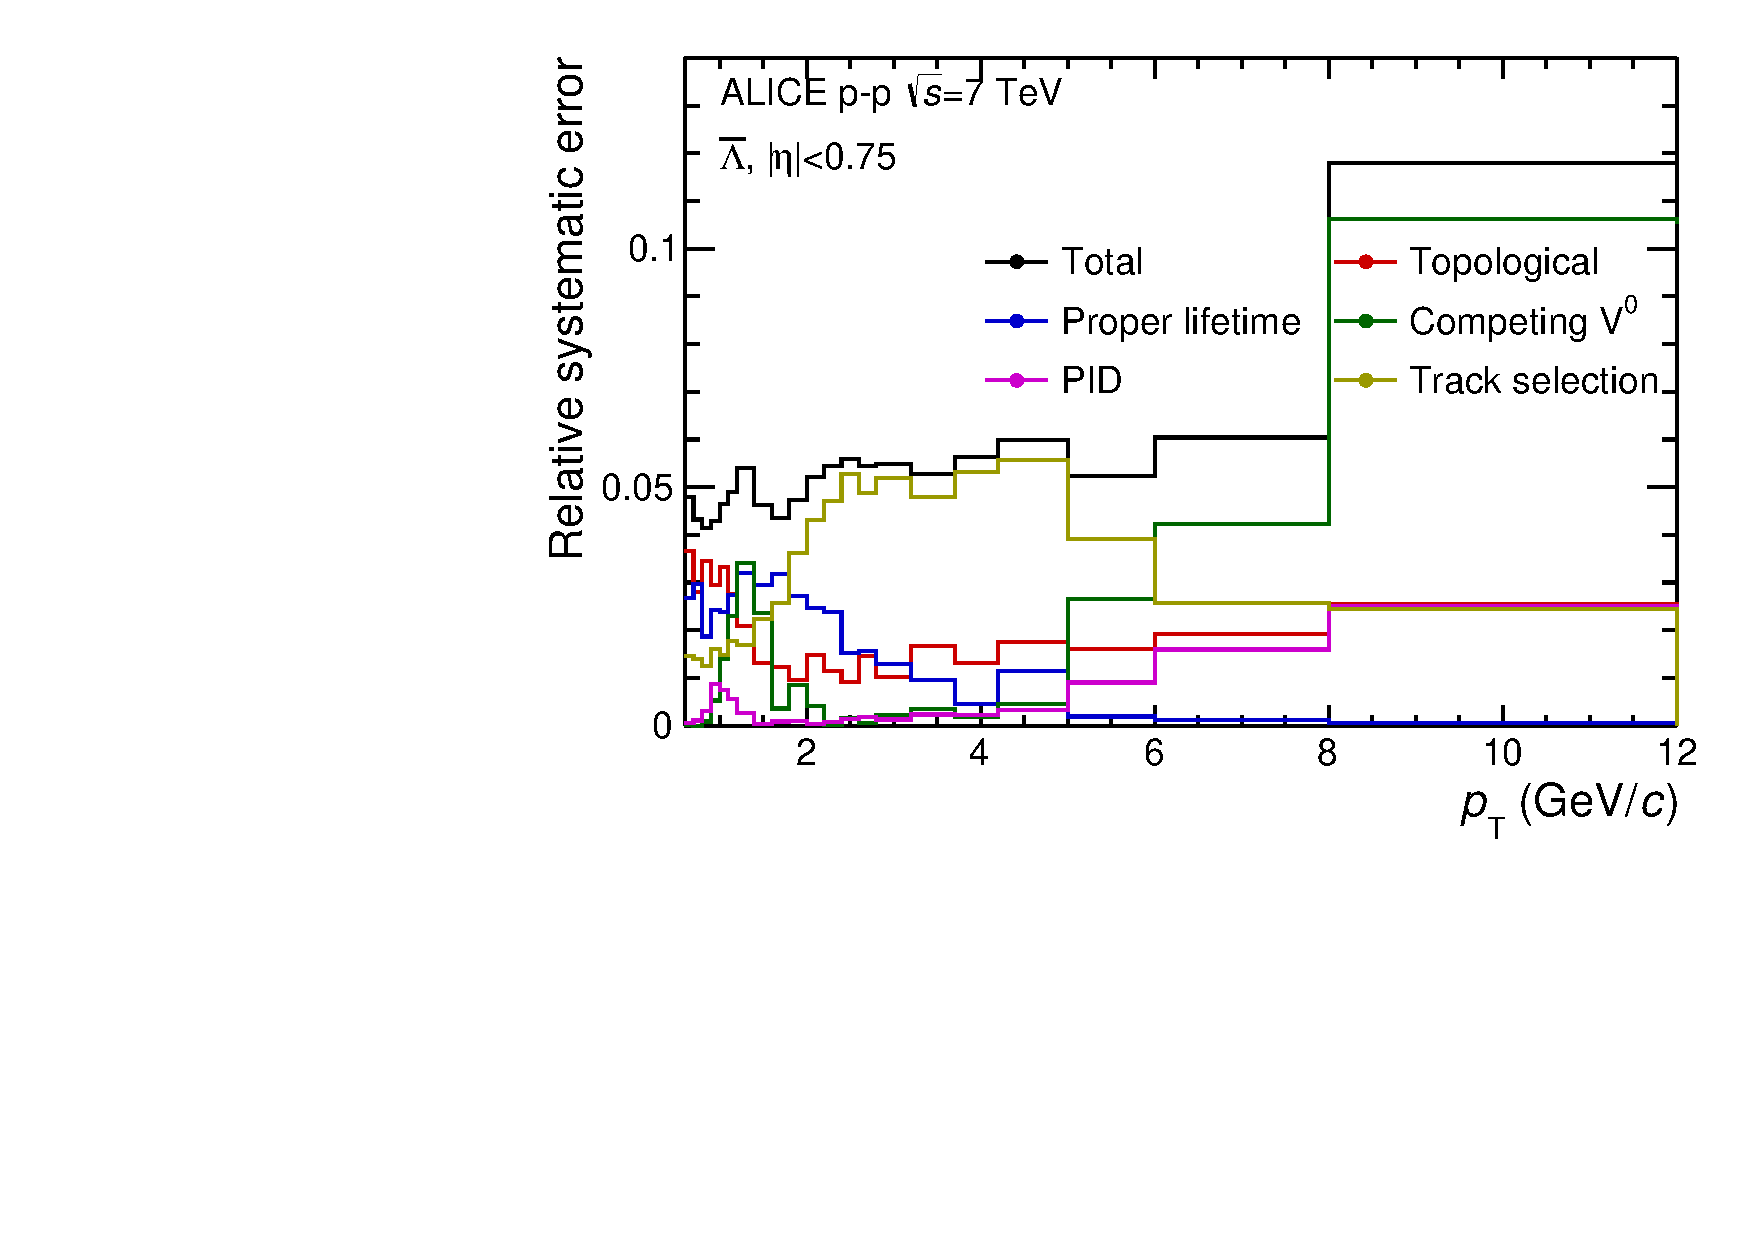
\includegraphics[width=.49\textwidth]{cSystIncl_AntiLa}
	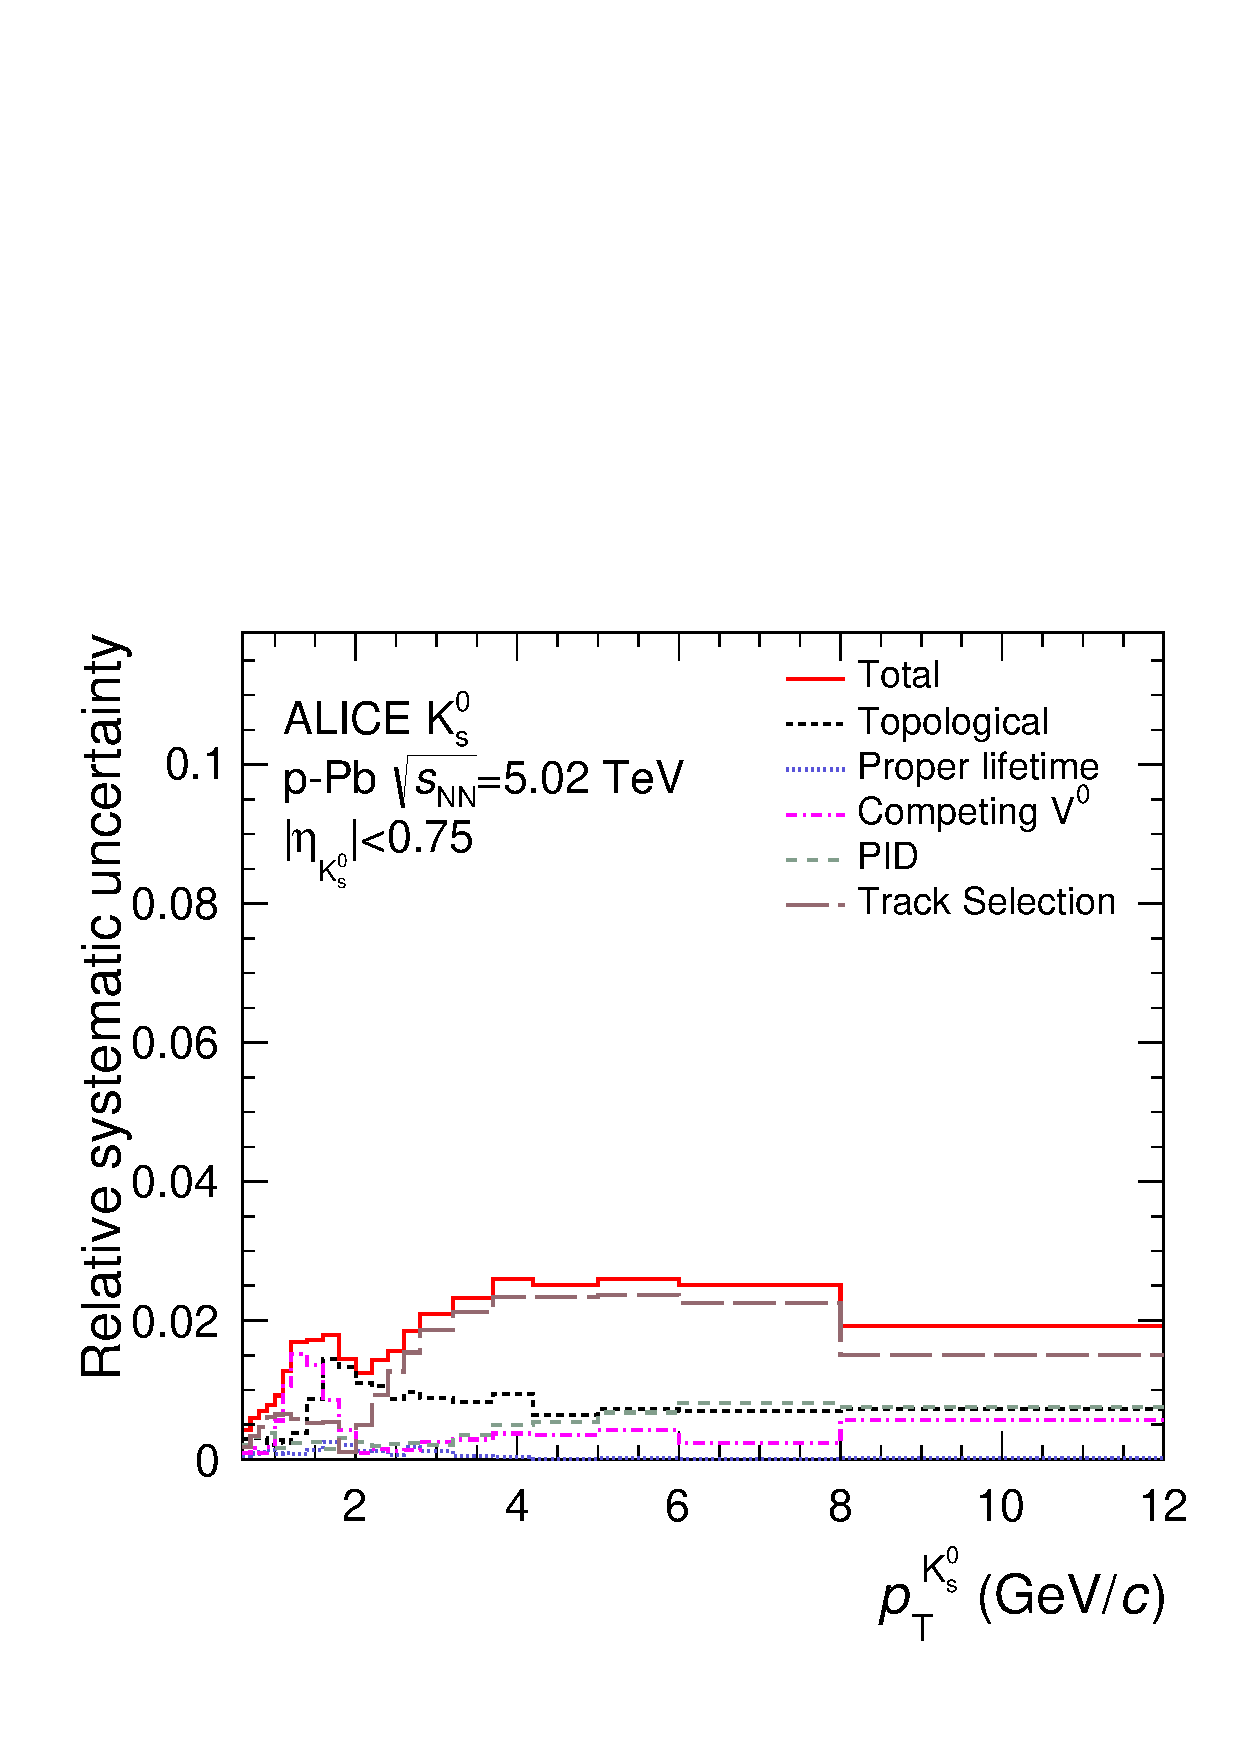
\includegraphics[width=.49\textwidth]{Inclusive_K0s_syst_uncert.pdf}
	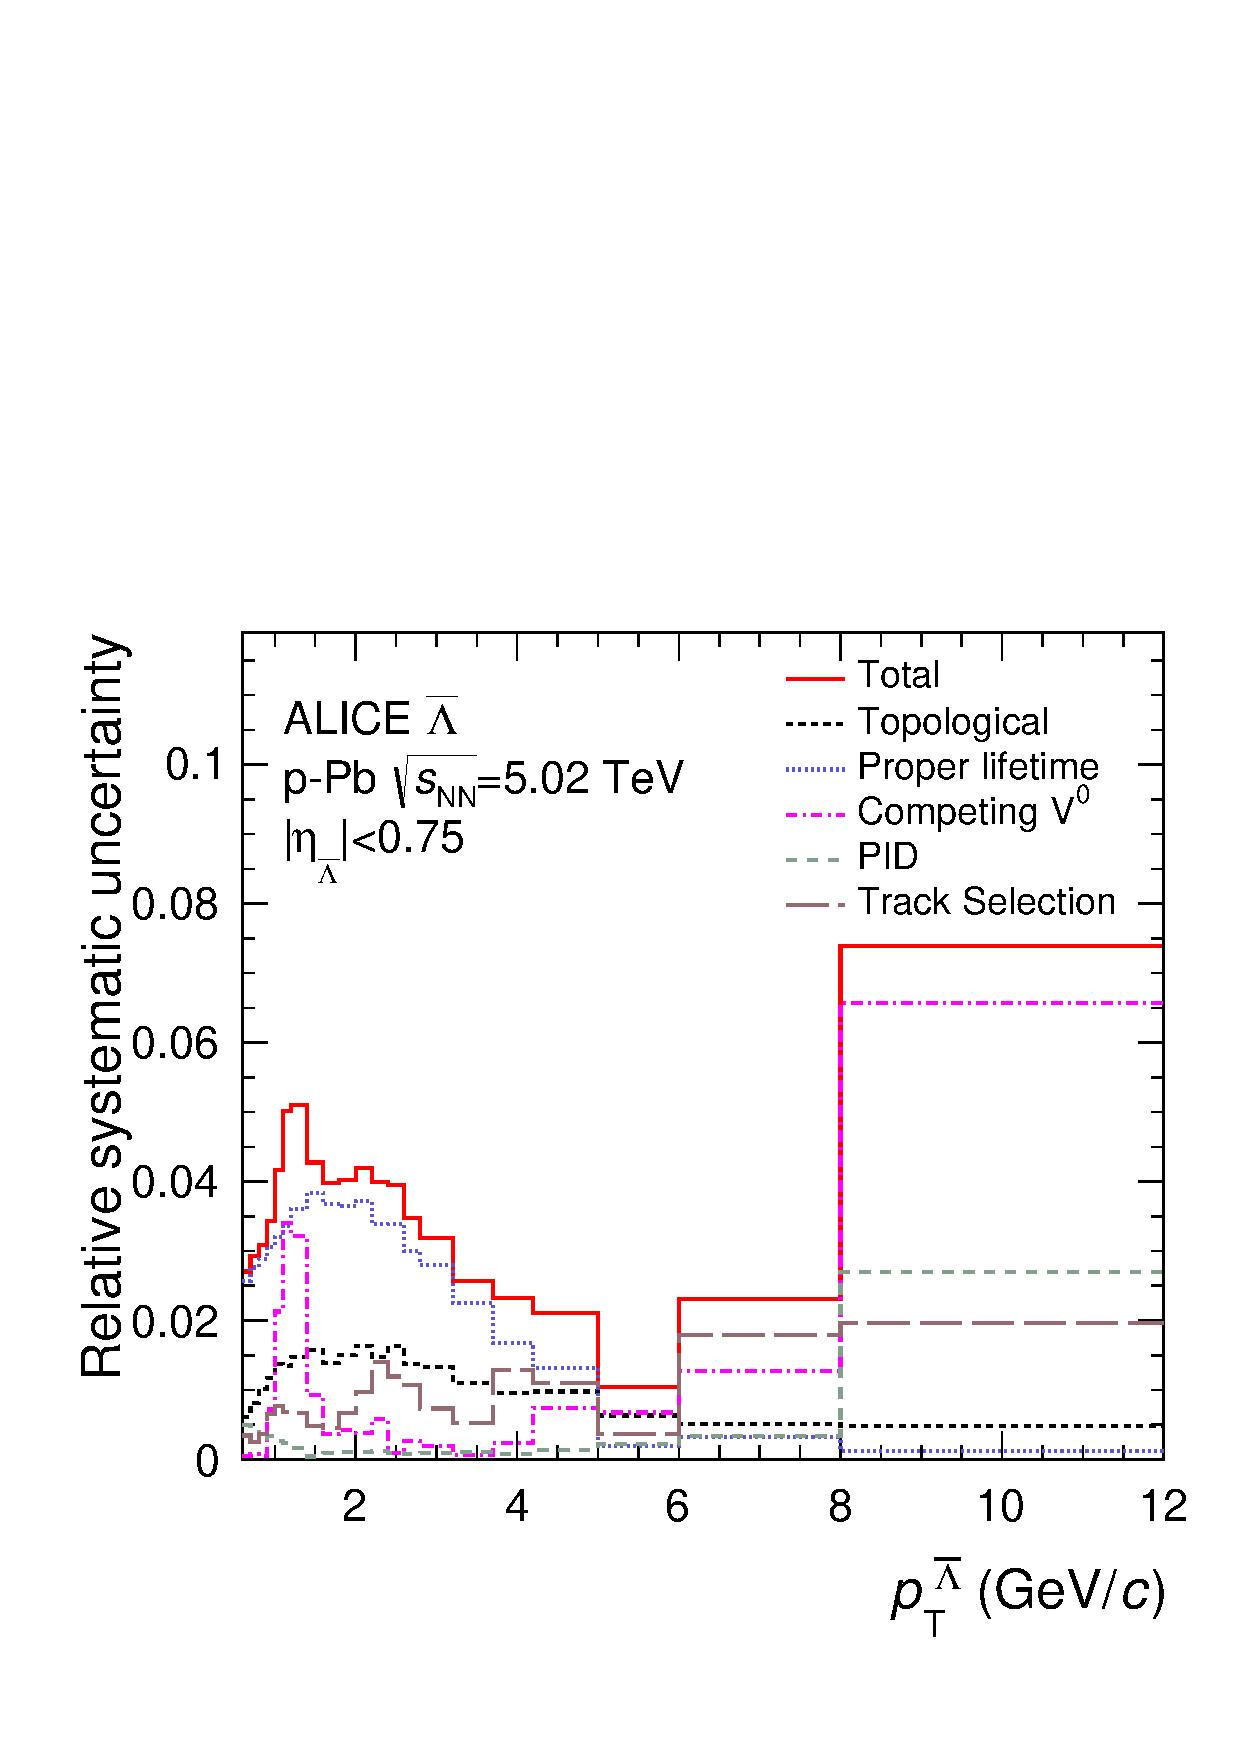
\includegraphics[width=.49\textwidth]{Inclusive_AntiLambda_syst_uncert.pdf}
	\caption{Systematic uncertainties on \Vzero\ particle spectrum (left: \ks, right: \alda) as a function of their transverse momentum (see text for details). The systematic uncertainties associated to the \lda\ yield (not shown) are largely similar to \alda. \ask{MP: Uncertainties should be smoothed (local minima in some cases are unphysical).}}
	\label{fig:systUncert}
\end{figure}

%%%%%%%%%%%%%%%%%%%%%%%%%%%%%%%%%%%%%%%%%%%%%%%%%%%%%%%%%%%%%%%%%%%%%
%%\subsubsection{Uncertainty in UE \Vzero\ estimation}
%%\ask{sections below need more quant. and phrasing to be checked; also add a summary figure as a function \pt}

{\bf Uncertainty on the yields in the underlying event.} Two main sources of uncertainties originating from the mis-association of \Vzero particles with UE were considered: i) the \Vzero\ particle was found outside the selected jet and classified as UE particle; however, it may have originated from a physical jet outside the fiducial acceptance for jets considered in the analysis and/or from a {\it true} low-\pt\ jet, below the considered thresholds; and ii) the \Vzero\ particle originates from a true high-\pt\ jet; however, due to the finite detector efficiency the jet has not been reconstructed above the considered \pt\ threshold.

The uncertainty on the UE \Vzero\ density has been estimated using the two variations of the UE estimators: the {\it outside cone} (OC) and the {\it non-jet events} (NJ).
The OC and the NJ estimators encapsulate the maximum deviation in the yield of UE particles and the difference of the reconstructed \Vzero\ yields in OC and NJ has been included as the additional systematic uncertainties on the density of particles within the jets (JC).
The uncerainty is largest for low-momenta particles ($< 2~\gevc$) reaching up to 30\% but drops rapidly with \pt\ to negligible values for $\pt > 6~\gevc$.

%%%%%%%%%%%%%%%%%%%%%%%%%%%%%%%%%%%%%%%%%%%%%%%%%%%%%%%%%%%%%%%%%%%%%

%%\subsubsection{Jet reconstruction and jet selection}

{\bf Uncertainty on yields in jets.} The systematic uncertainty originating from the selection of the jet \pt\ were estimated by repeating the analysis with jet \pt\ varied around the chosen thresholds of 10 and 20~\gevc\ by 2~\gevc.
This variation accounts for jet resolution due to detector effects and the fluctuations of the event background density as reported in \cite{Adam:2015hoa}.
For jets with $\ptch>10~\gevc$ at low momenta ($\ptvzero<2\gevc$) it reaches up to 10\% while it is about 20\% for jets of $\ptch>20~\gevc$.
%% The uncertainty remains almost constant of about 5\% for $\ptvzero > 2~\gevc$ independently of the $\ptch$. \ask{check numbers}
The uncertainty remains almost constant of about 3\% for $\ptvzero > 2~\gevc$ for jets $\ptch>10~\gevc$ and about 5\% for jets $\ptch>20~\gevc$.

\begin{figure}[htbp]
	\centering
	%%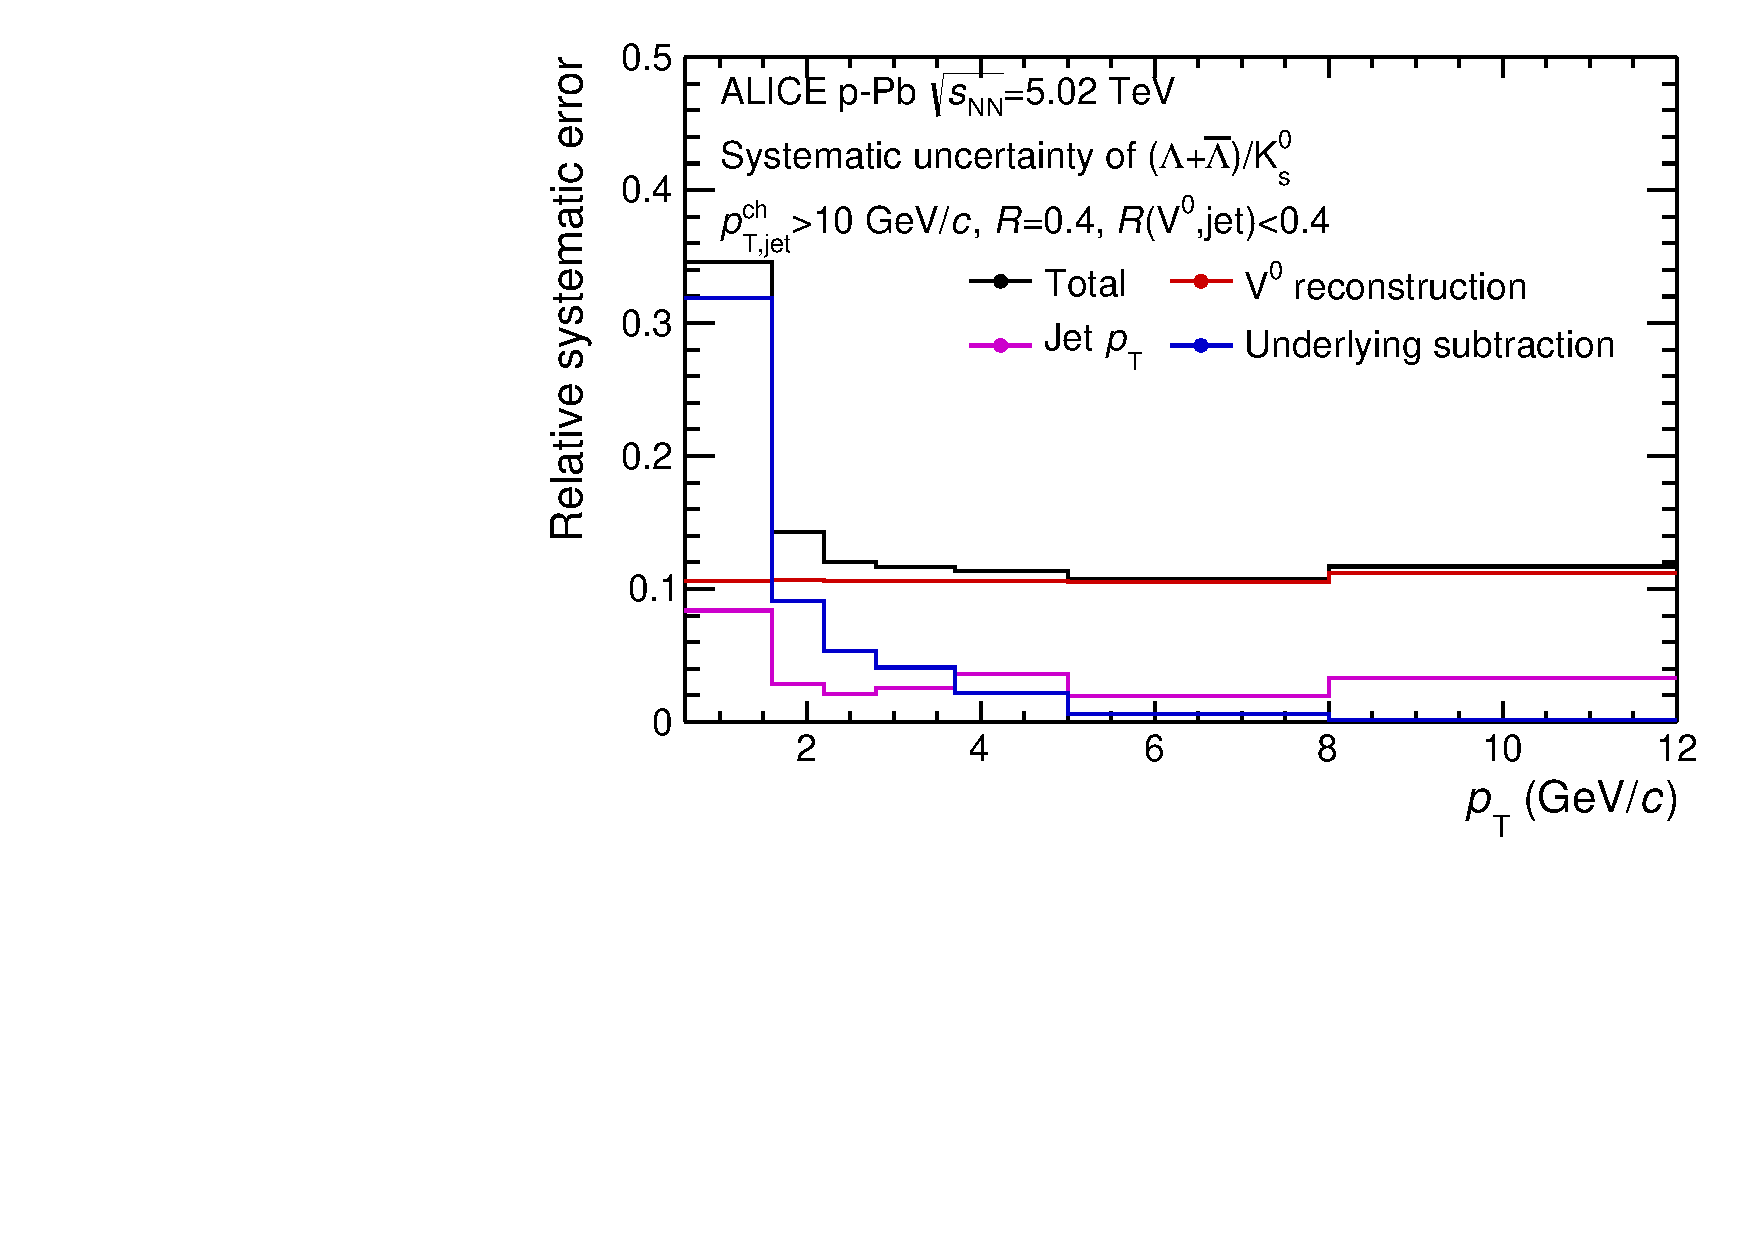
\includegraphics[width=0.47\textwidth]{cSystInJE_RatioV_Ptj10}
	%%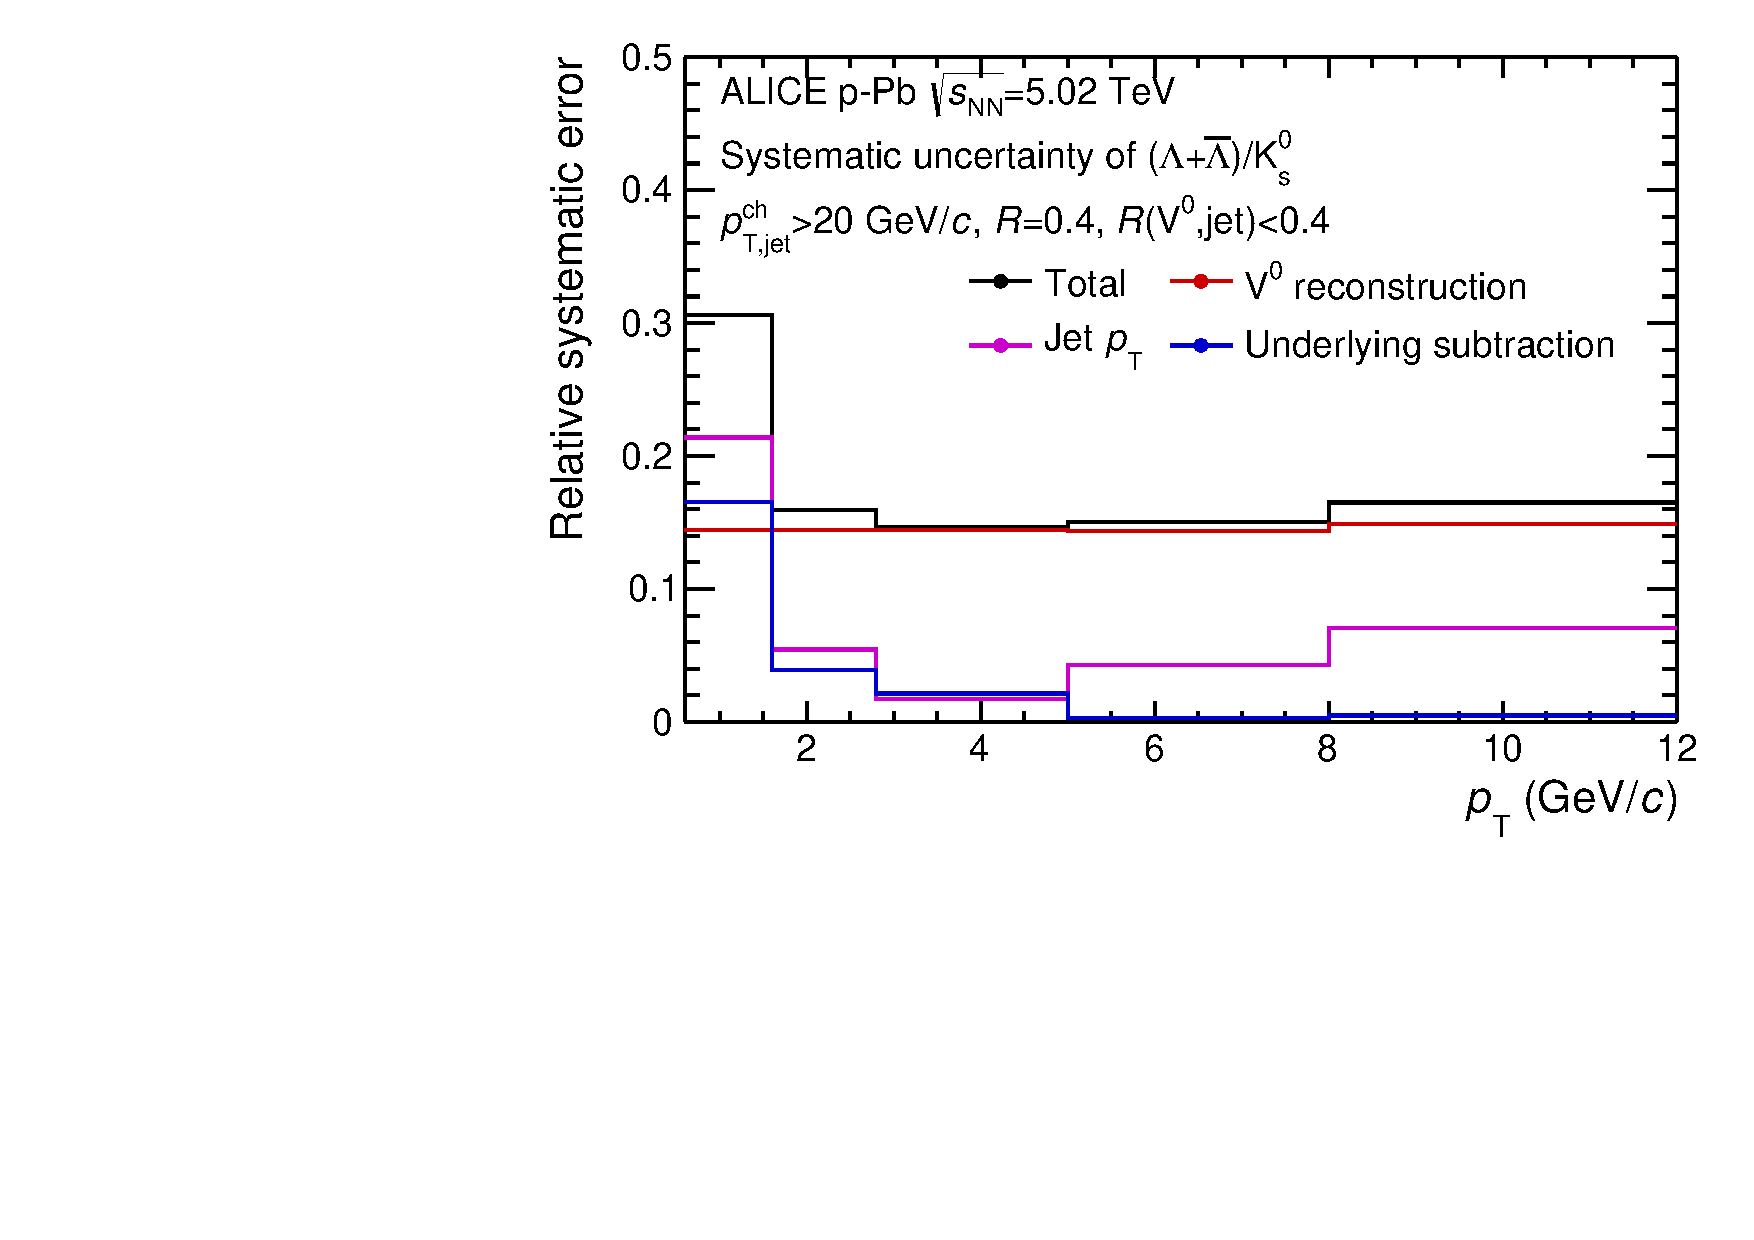
\includegraphics[width=0.47\textwidth]{cSystInJE_RatioV_Ptj20}
	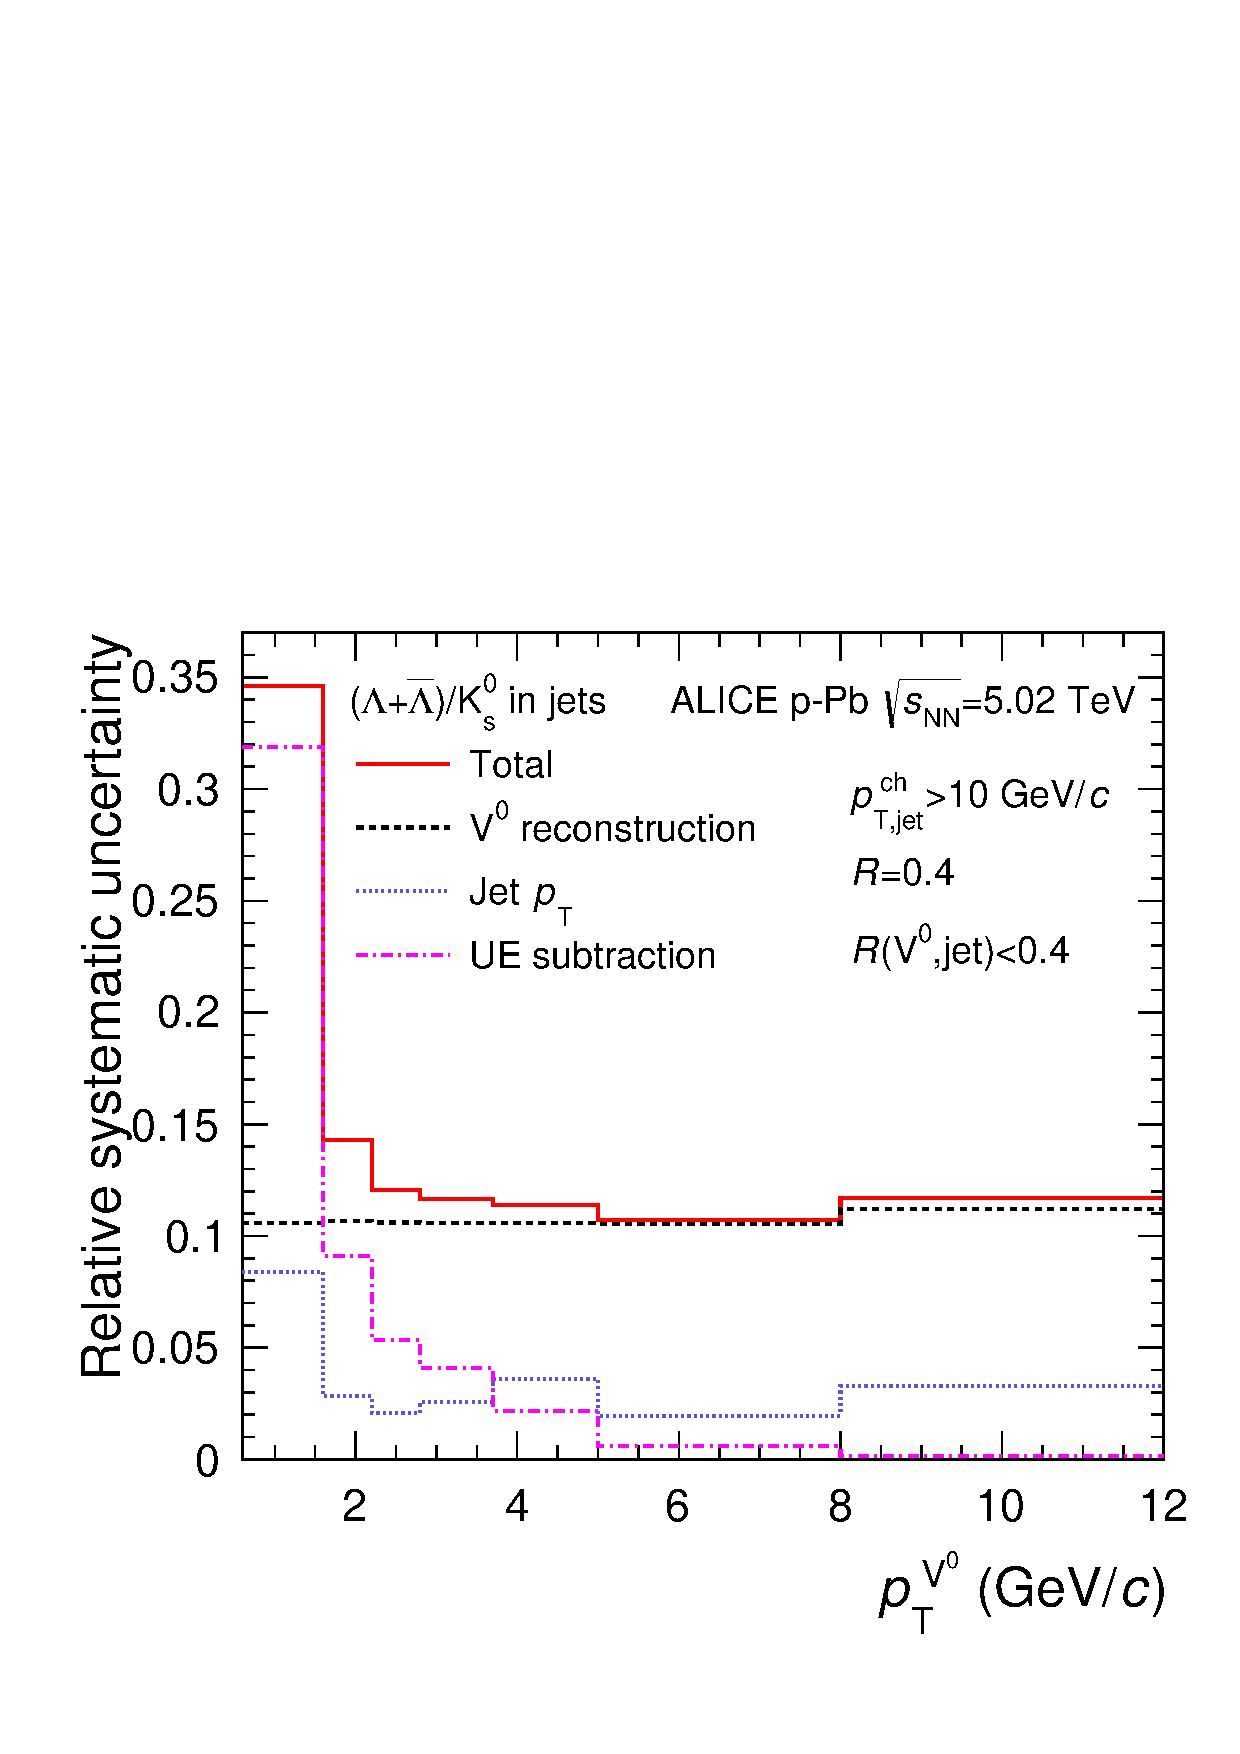
\includegraphics[width=0.49\textwidth]{L2K_in_jet_syst_uncert_10GeV.pdf}
	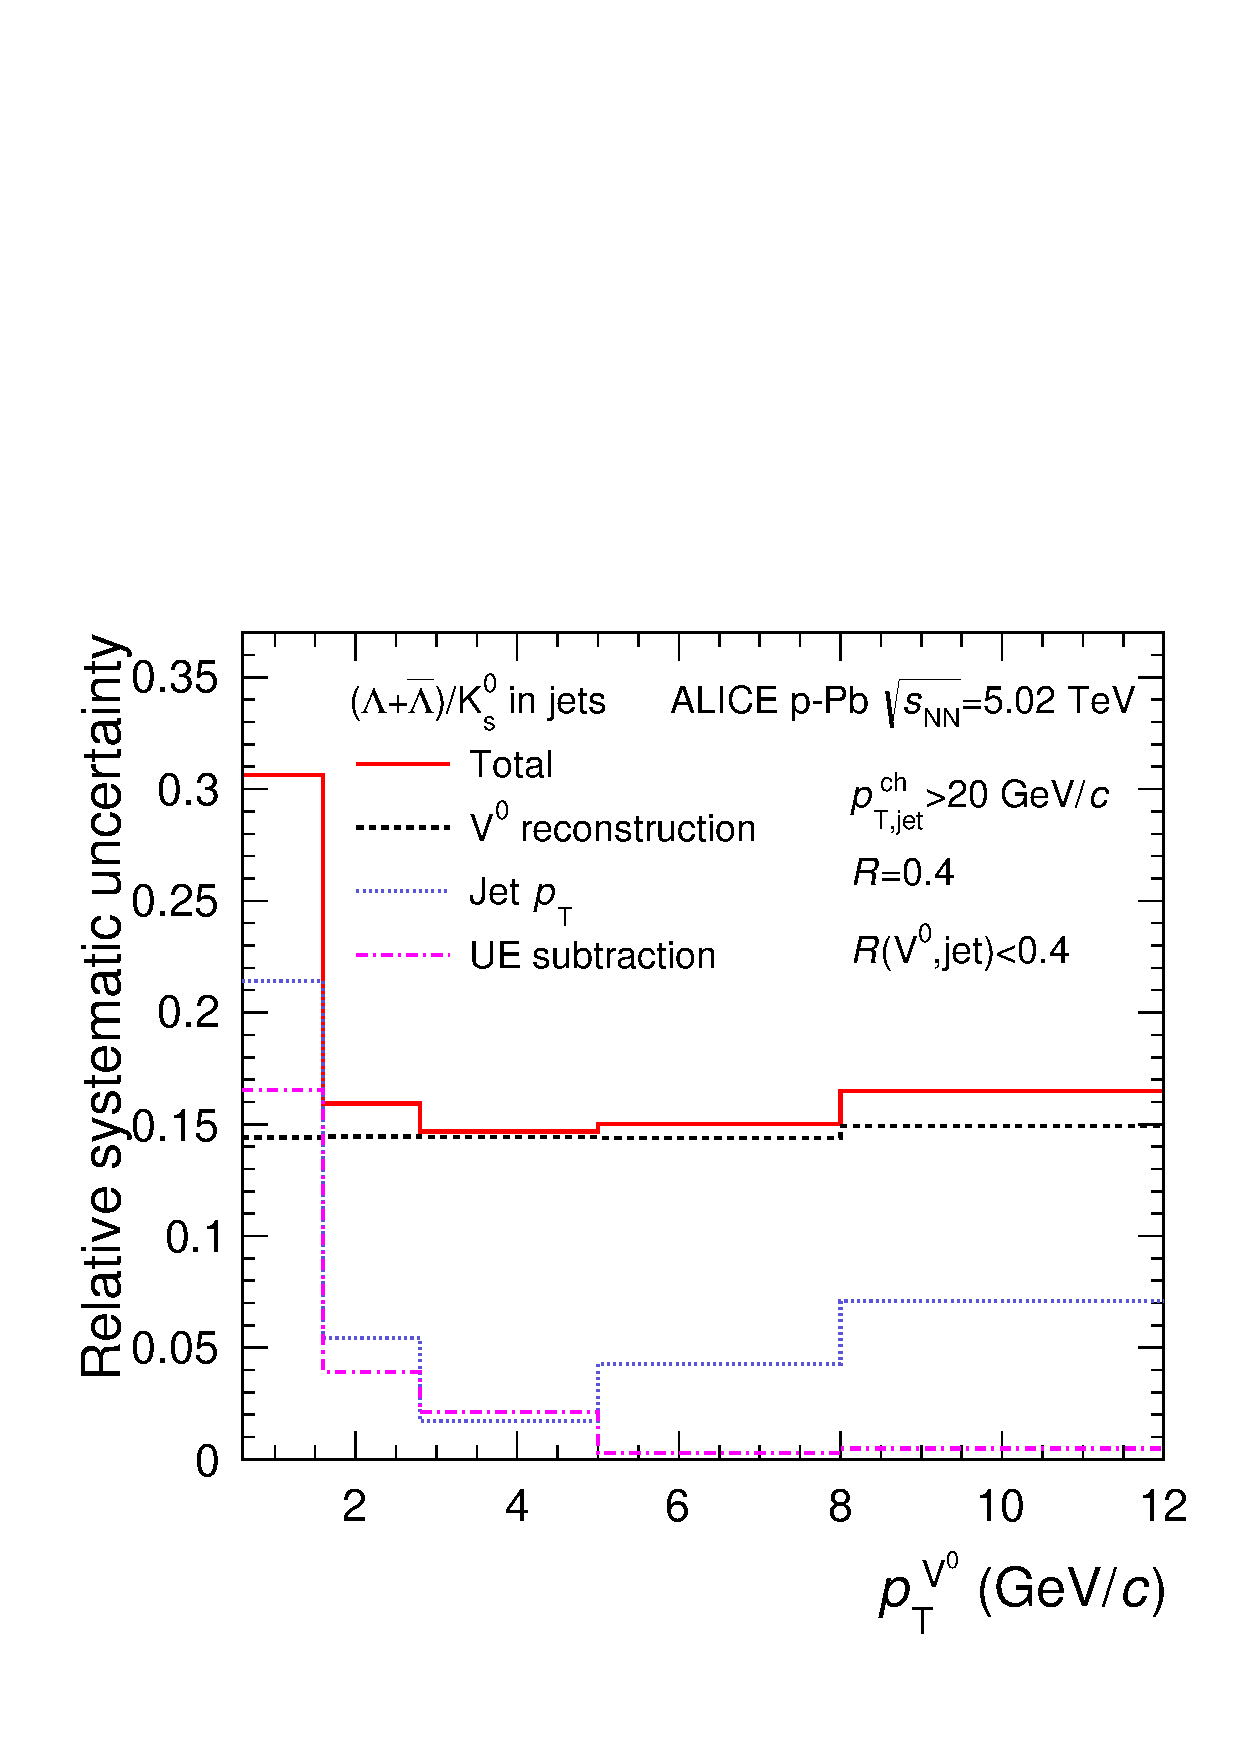
\includegraphics[width=0.49\textwidth]{L2K_in_jet_syst_uncert_20GeV.pdf}
	\caption{Relative systematic uncertainty on the ratio of \lda\ and \ks\ spectrum within $R=0.4$ anti-\kt\ jets for $\ptch>10~\gevc$ (left) and $\ptch>20~\gevc$ (right) as a function of particle \pt. Three contributions to the total uncertainty are shown: uncertainty on \vzero\ reconstruction, uncertainty on the underlying event subtraction, and uncertainty on the jet momentum scale and momentum resolution. }
	\label{fig:systUncertRatio}
\end{figure}

{\bf Uncertainty on the \lda/\ks\ ratio.} The uncertainties on \Vzero\ yields, material budget and feeddown correction are propagated to the ratio quadratically.
The uncertainties related to~ the jet \pt\ and UE estimation are obtained by calculating the deviation of ratios between the default analysis and various selections.
%%\ask{Jana: Add explanation how the systematic uncertainties were propagated to the lambda/K0S ratio.}
Figure \ref{fig:systUncertRatio} shows the relative systematic uncertainties on the $(\lda+\alda)/(2\ks)$\ ratio reconstructed within $R=0.4$ jets with $\ptch > 10~\gevc$ and $\ptch > 20~\gevc$ as a function of particles \pt.
For the $\ptch > 20~\gevc$ the total uncertainty is about 16\% and is largely independent of particle \pt\ with the largest contribution of 14\% originating from the uncertainty on \Vzero\ reconstruction.

%%\ask{what about jet finding efficiency? - what is the rec. efficiency and how it varies with the fragmentation model? => estmated from the jets where no jets was found... the UE subtraction -> jets where only particles produced are \lda\ and/or \ks\ ?}

%%%%%%%%%%%%%%%%%%%%%%%%%%%%%%%%%%%%%%%%%%%%%%%%%%%%%%%%%%%%%%%%%%%%%

\section{Results}
\label{sec:Results}

\subsection{\pt-dependent densities of \vzero\ particles}

The fully corrected densities of \ks\ and the sum of \lda\ and \alda\ particles associated to a hard scattering tagged by a jet are shown in Fig. \ref{fig:rhov0}.
The per jet density within the jet cone (JC) is compared to the density for inclusive particles (without association to jets) and to the density in the perpendicular cones (PC).
In the case of inclusive particles the distribution is normalized to the product of the total number of events and the acceptance of the \vzero\ particles in a single event (full azimuth and $|\eta|<0.75$).
As expected, for both \ks\ and \lda\ particles the \pt\ dependence of the density within jets is much less steep as the as the high-\pt\ particles originate from jets.
The density in the PC selection is qualitatively similar to the inclusive distribution showing strong, steeply falling \pt\ dependence.
Both, the inclusive and the PC distributions show a rapid decrease with \pt\ reaching values more than an order of magnitude lower than the JC density for particle \pt\ exceeding $4~\gevc$.
This is consistent with an expectation that the high-\pt\ particles originate from jet fragmentation.

\begin{figure}[htbp]
	\centering
	%% 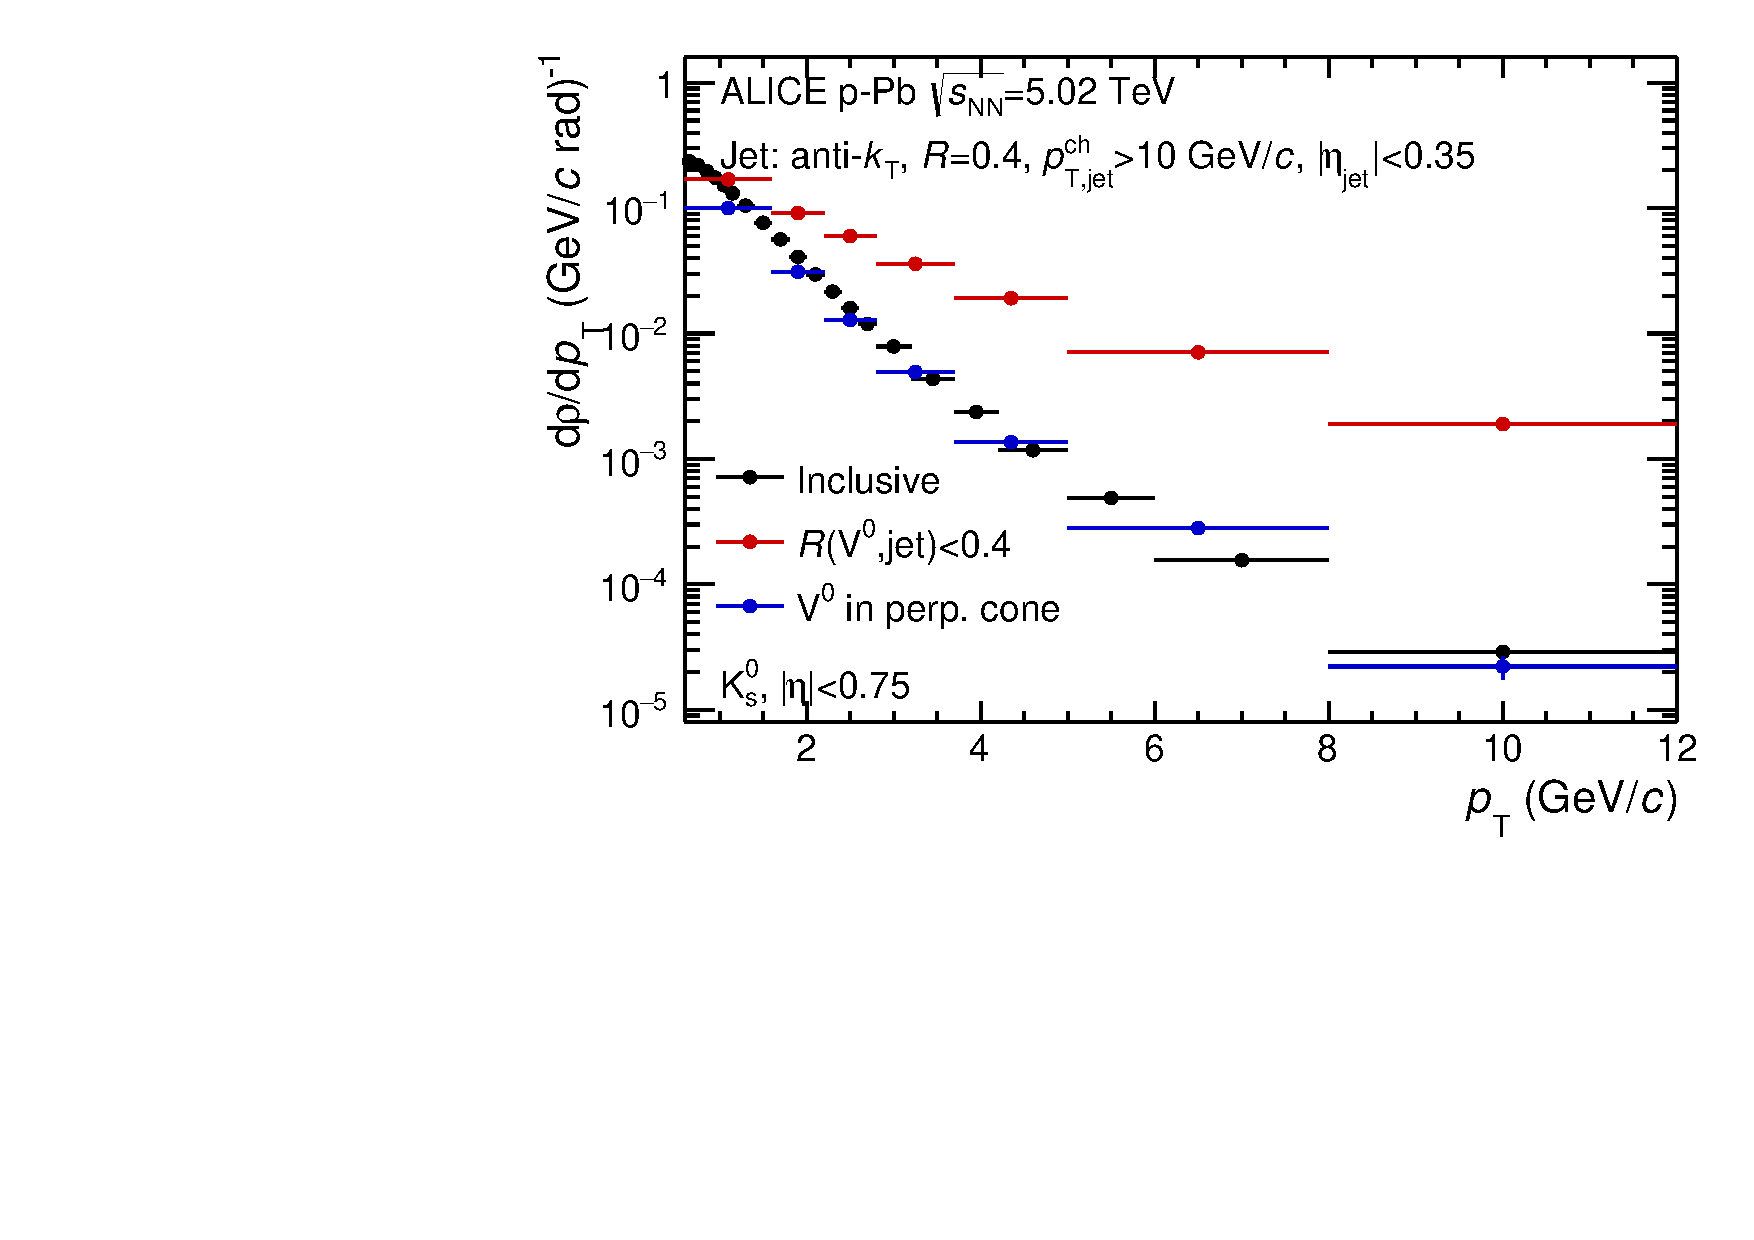
\includegraphics[width=0.47\textwidth]{cRho_Kshort_JE_JR04_JC04}
	%% 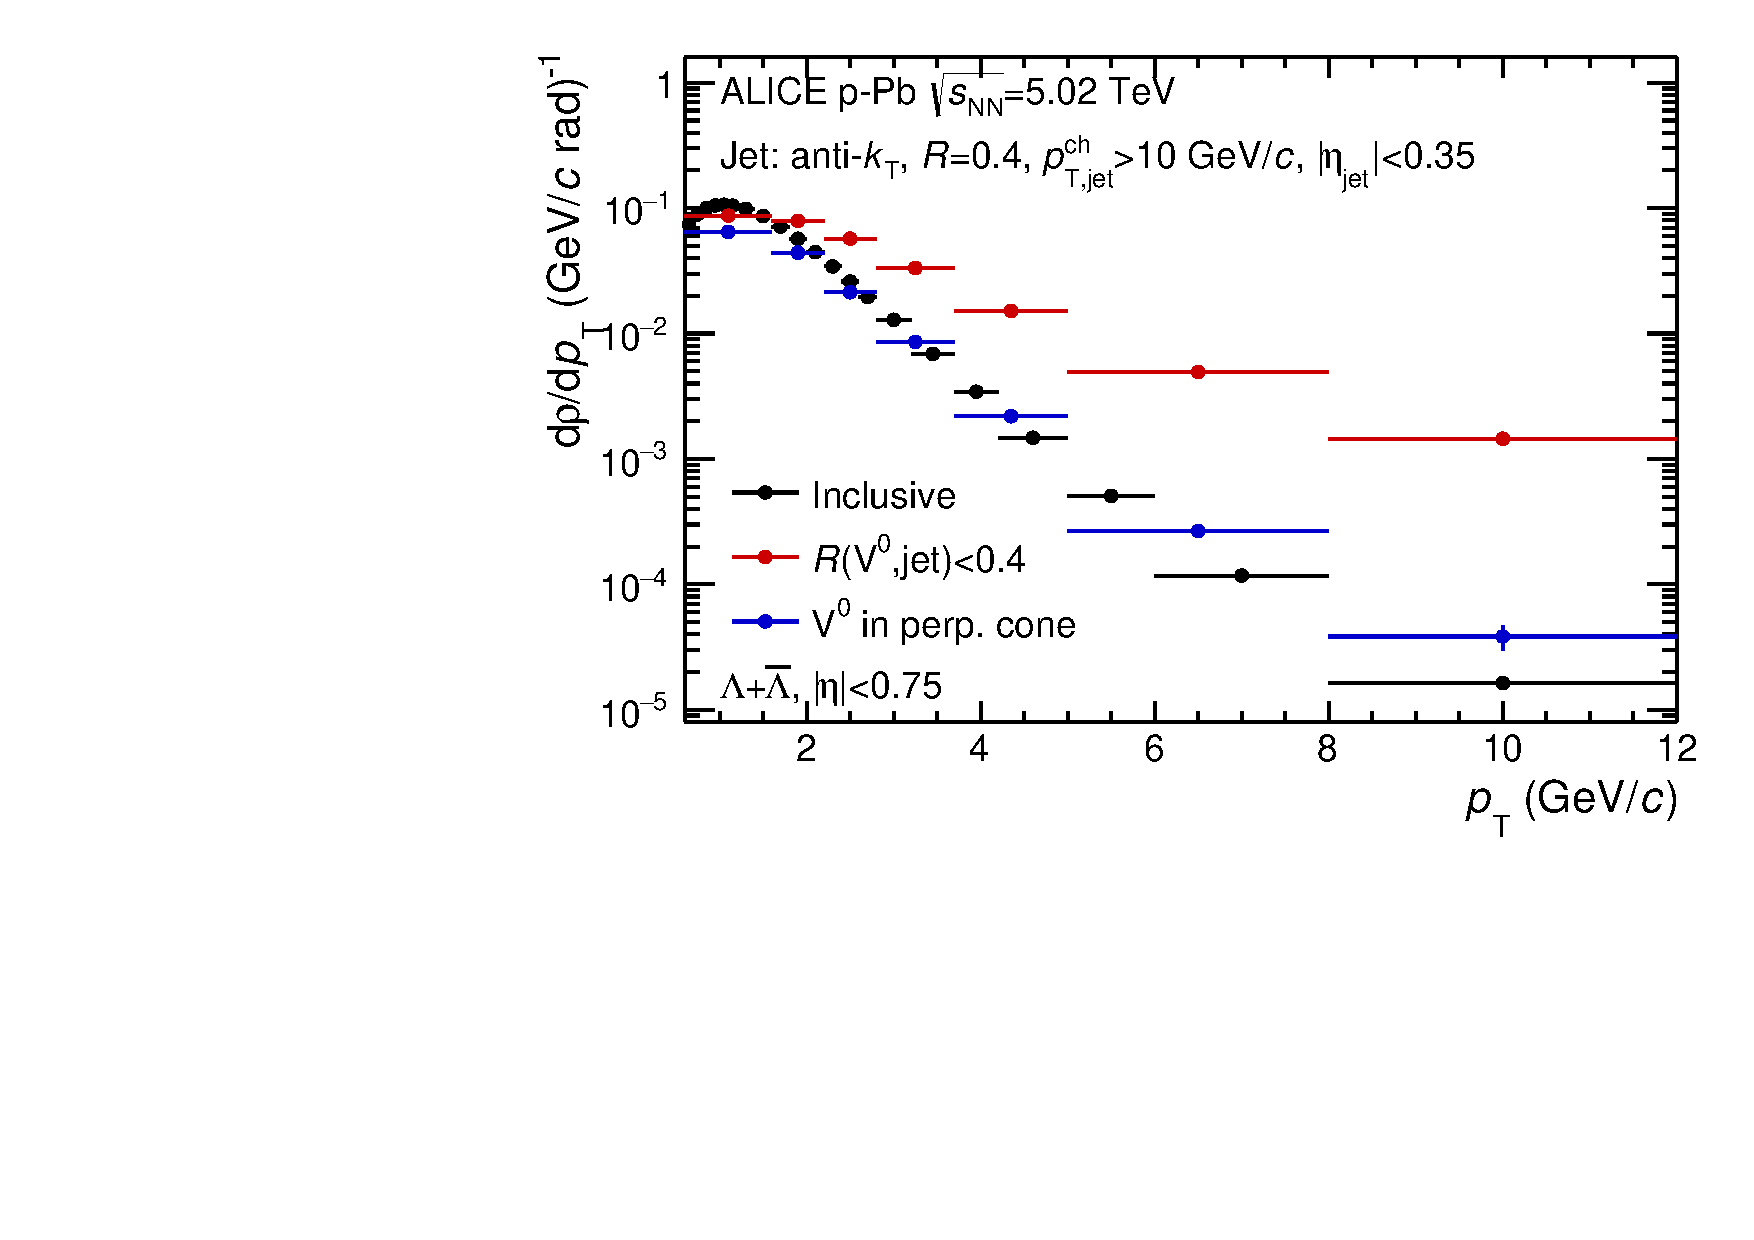
\includegraphics[width=0.47\textwidth]{cRho_Lambda_JE_JR04_JC04}
	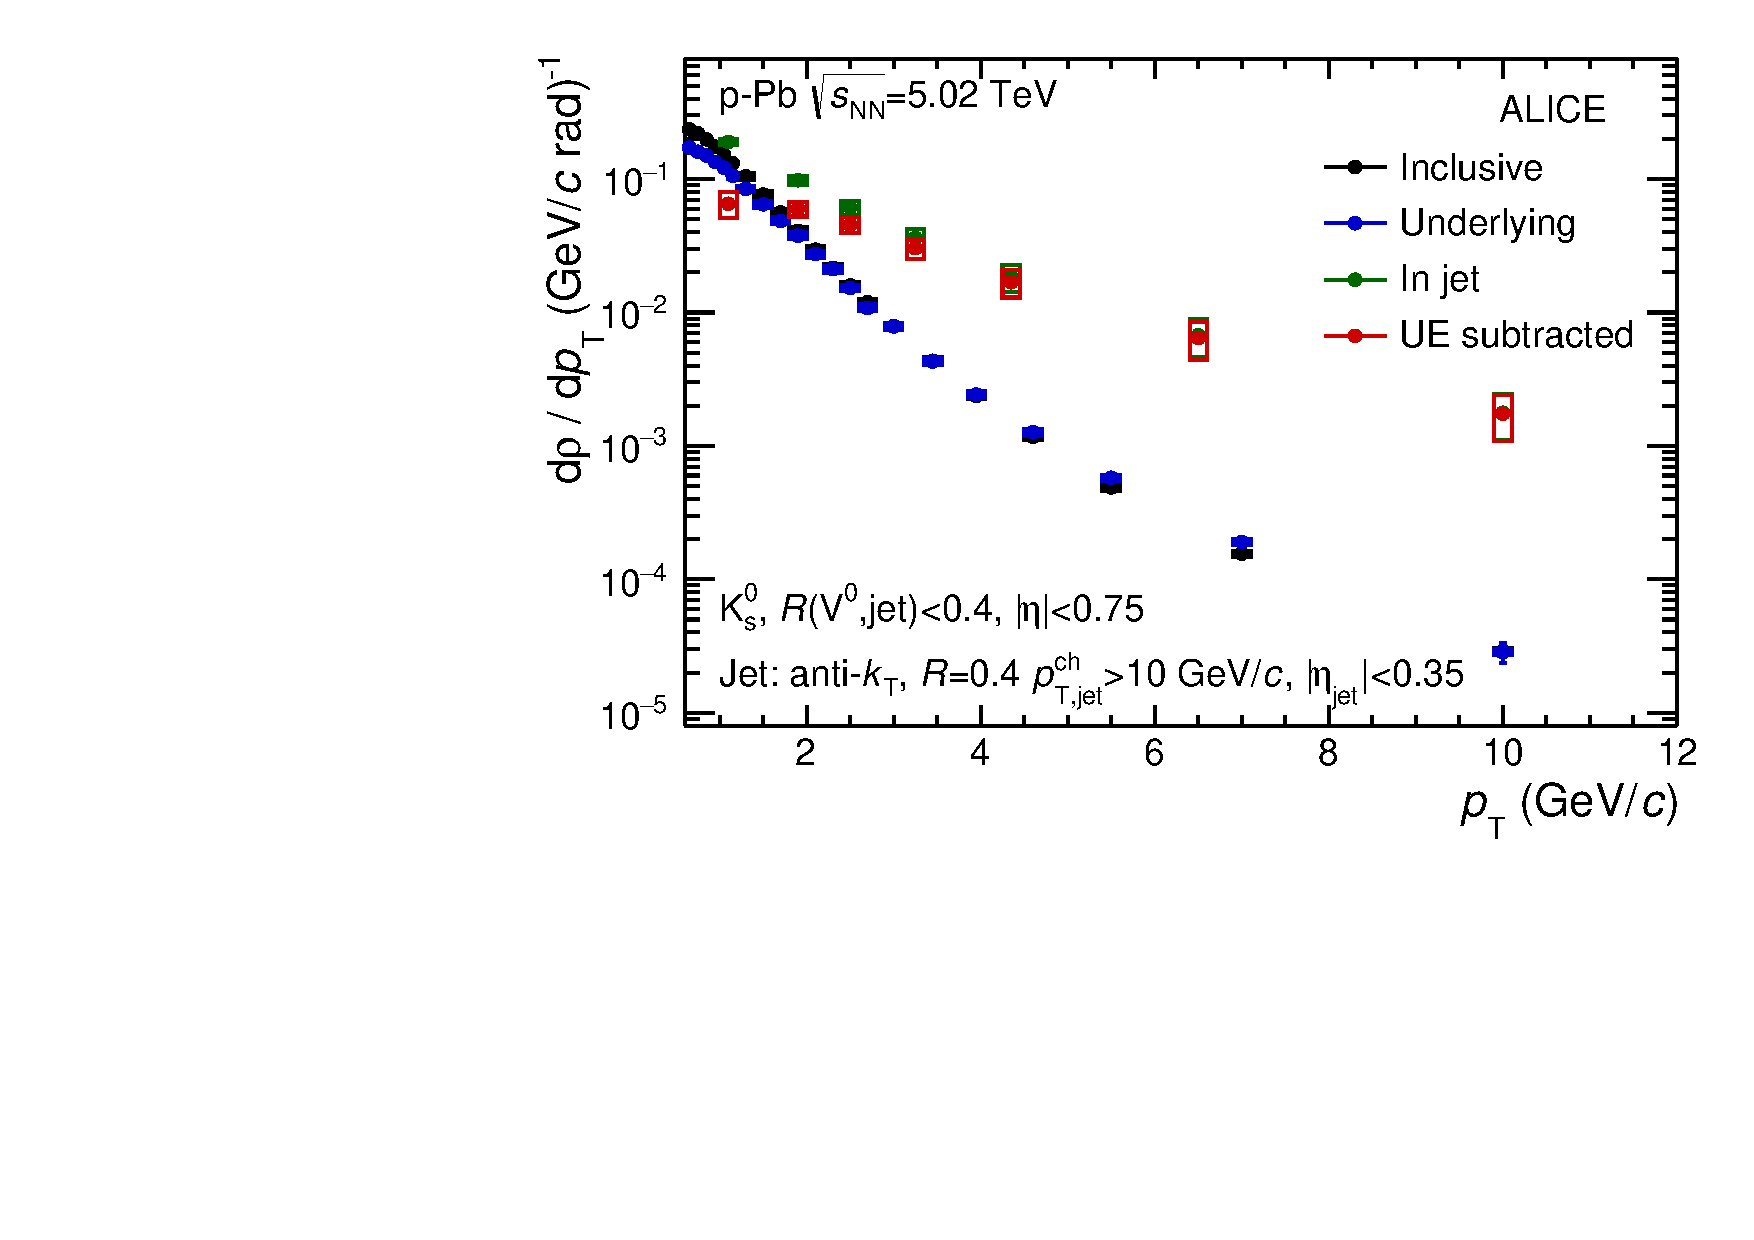
\includegraphics[width=0.47\textwidth]{cFig4a}
	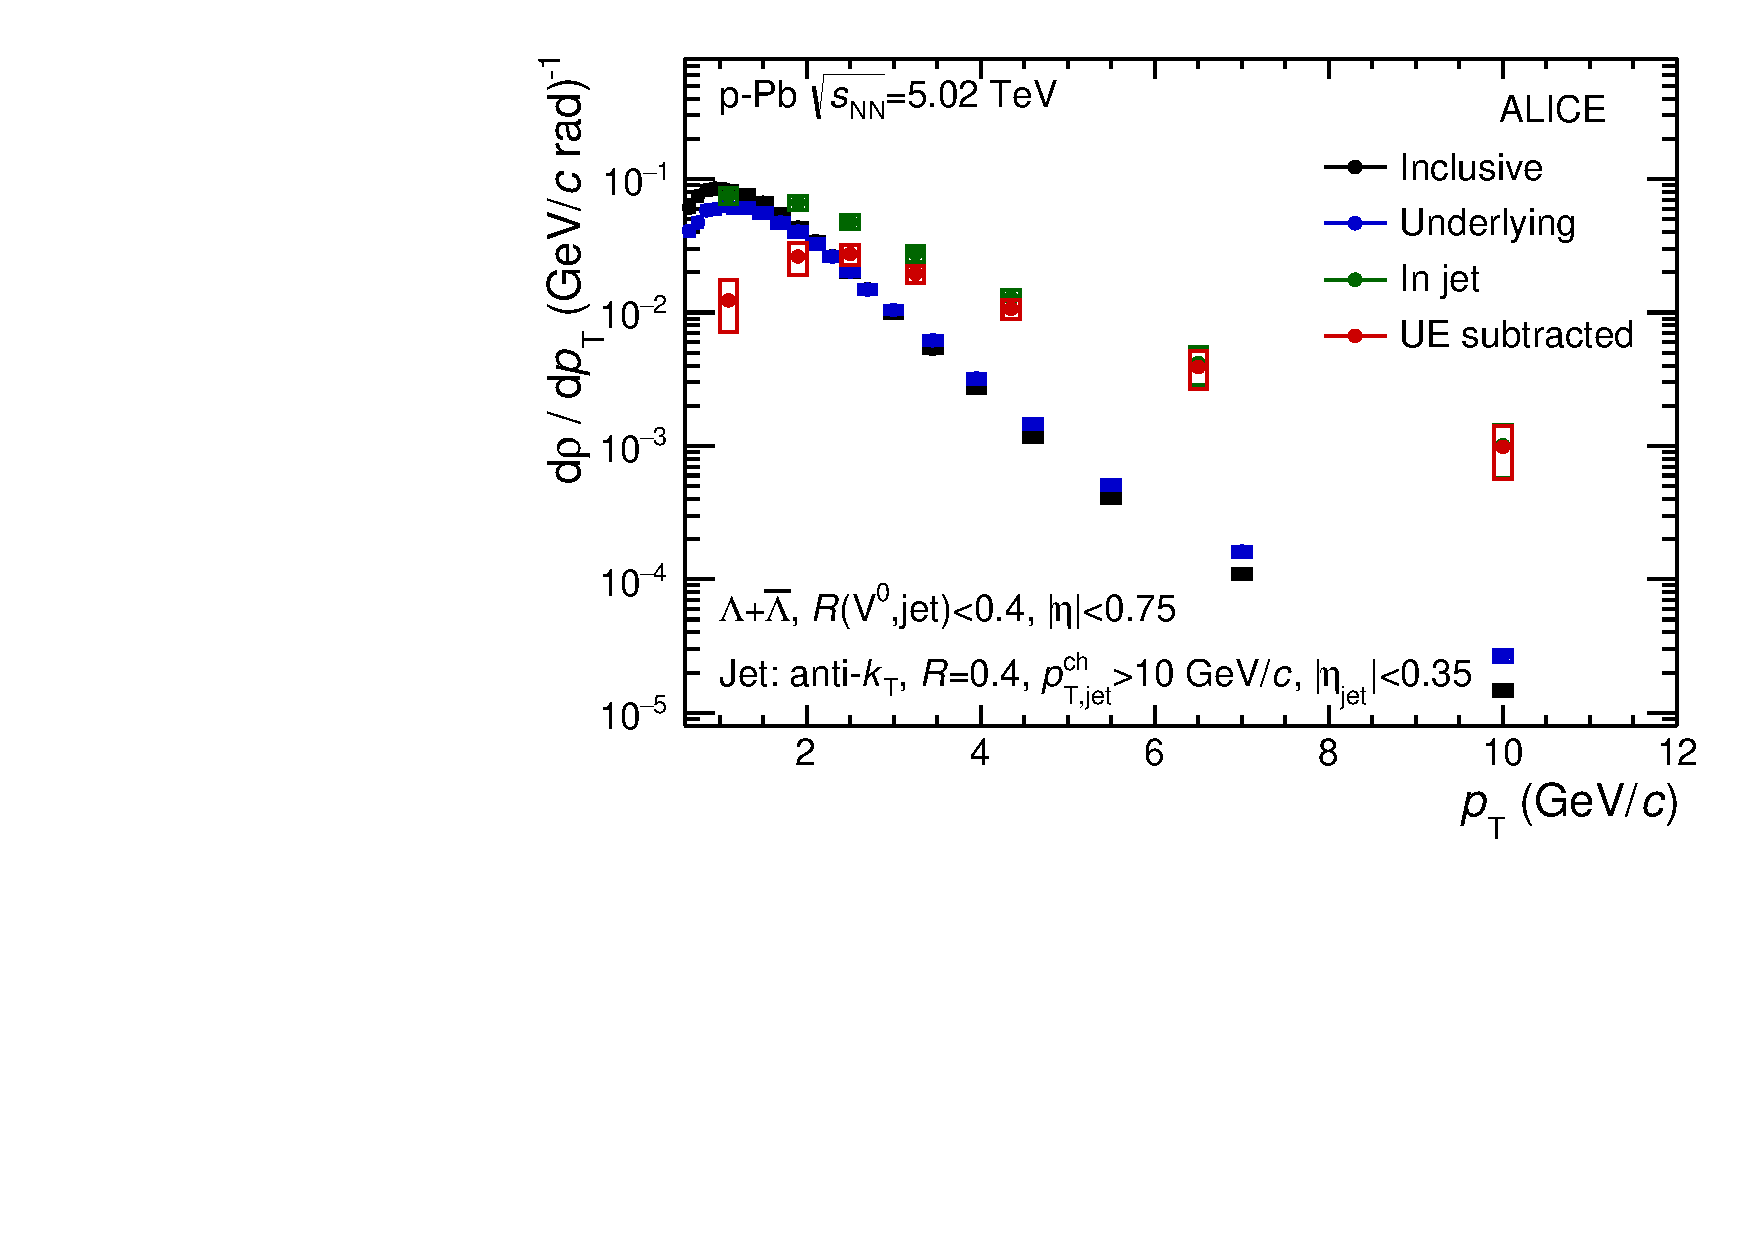
\includegraphics[width=0.47\textwidth]{cFig4b}
	\caption{Differential density of particles \drhodpt\ (see Eq. \ref{eq:defv0rho}) in p-Pb collisions at \sqrtsnn{5.02} for \ks\ (left), and the sum of \lda\ and \alda\ (right). The density is shown for three selections: inclusive particles from minimum bias events, particles within anti-\kt\ jets ($\ptch>10~\gevc$) with $R=0.4$ and particles within the perpendicular cones (PC) in events containing jets.}
	\label{fig:rhov0}
\end{figure}

\subsection{$(\lda+\alda)/(2\ks)$ ratios}
%the ratio is not sensitive to the jet resolution parameter $R$

Ratios of \lda\ and \ks\ yields can be obtained by dividing the normalized density distributions.
In the following the sum of \lda\ and \alda\ densities is divided by twice the density of \ks.
As no significant difference was found for different jet resolution parameters $R$ the results are presented as the average of results obtained with $R$ of 0.2, 0.3, and 0.4.
Figure \ref{fig:LKR} shows the ratio for the raw JC selection (JC yield without the UE background subtraction) as a function of the distance from the jet axis \rvzerojet.
The ratio is shown for three momentum bins: the low-\pt\ ($0.6 <\pt <1.8~\gevc$), intermediate \pt\ ($2.2 < \pt < 3.7~\gevc$), and the high-\pt\ ($4.2 < \pt < 12~\gevc$).
The ratio as a function of \rvzerojet\ at low-\pt\ remains approximately constant at about $0.2$ independent of the distance to the jet axis and that is the case even at large distances of $\rvzerojet > 1.2$.
This value is consistent with the inclusive measurements in \pPb\ collisions, but also in \pp\ and peripheral \PbPb\ collisions were effects related to the collective expansion of the system are either not-present or small \cite{Abelev:2014uua}.

Conversely the intermediate-\pt\ selection shows an increase of the ratio from about $0.3$ when evaluated close to the jet axis to values of about $0.6$ at \rvzerojet\ distances of about $0.5$.
For distances $\rvzerojet > 0.5$ the ratio remains constant.
The ratio of $0.6$ is consistent with the inclusive measurement in \pPb\ collisions \cite{Abelev:2013haa} and this \pt\ region is where the enhanced \lda/\ks\ ratio in the inclusive measurements was found the largest.
We stress that for the results shown in Fig. \ref{fig:LKR} the UE backgrounds were not subtracted.
Therefore the evolution of the ratio as a function of the distance from the jet axis demonstrates how the two sources UE and jet compete.
The lack of enhancement (values consistent with \pp\ collisions) close to the jet axis indicate that the enhanced \lda/\ks\ ratio is not associated with the jets.
%%The increase to the inclusive  but rather a feature of the soft part of the event.

In each of the momentum bins the ratio is dominated by the lower edge of the selection window due to steeply falling particle \pt\ spectrum.
This is especially the case for the high-\pt\ selection where the dominating component originates from \pt\ of about $4.5~\gevc$ and the \rvzerojet\ dependence at high-\pt\ is similar to intermediate \pt. The ratio at high-\pt\ accociated to jets is discussed below.

%%%%
The right panel of Fig.~\ref{fig:L2Kratio} shows the ratio of \lda\ to \ks\ as a function of particle \pt\ for four selections: the inclusive particles, the particles from the PC selection, and two JC selections for jet \pt\ of $10$ and $20~\gevc$ averaged over three resolution parameters $R$ (0.2, 0.3, 0.4).
In this case JC selection, prior to forming the ratio, the UE density contribution obtained with the PC selection was subtracted for each particle species separately.
Additionally, for the results in Fig. \ref{fig:L2Kratio} every \Vzero\ particle was required to be close to the jet axis with its distance $\rvzerojet < 0.2$.
The inclusive and the PC distributions show the enhancement at \pt\ of about $3~\gevc$.
The ratio for the inclusive case is consistent with the measurement presented in \cite{Abelev:2013haa}.
The PC distribution above $2~\gevc$ reaches systematically higher values than the inclusive.
The $(\lda+\alda)/\ks$ ratio within jets is consistently lower than the inclusive case and approximately independent of \pt\ beyond $2~\gevc$.
In particular, the ratio for particles associated to the jet does not show a maximum at the intermediate \pt.
Clearly the enhancement of the ratio seen in the inclusive measurement is not present within jets.
This conclusion holds for both, 10~\gevc\ but also higher \pt\ ($20~\gevc$) jets.

\begin{figure}[htbp]
	\centering
	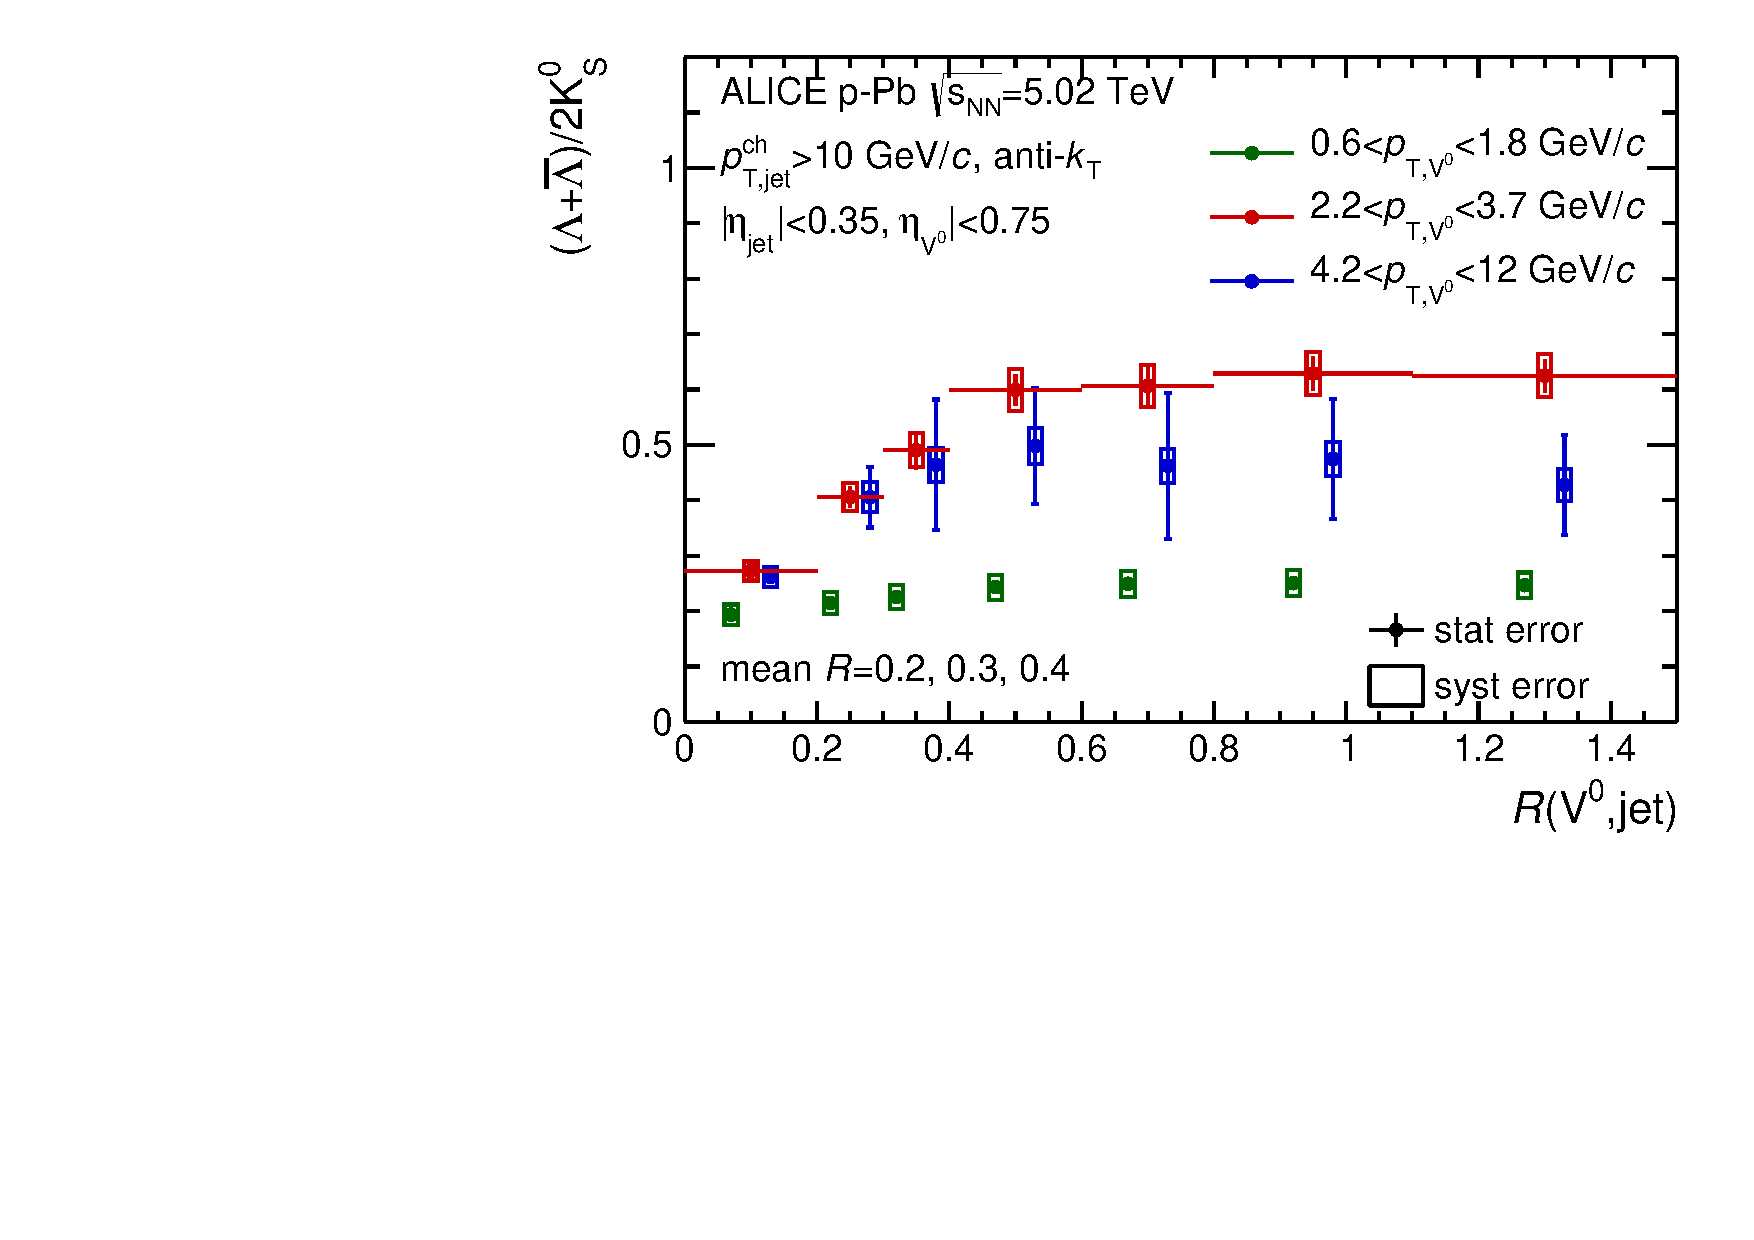
\includegraphics[width=0.47\textwidth]{cRatioV_VJ_Mean_PtJ10}
	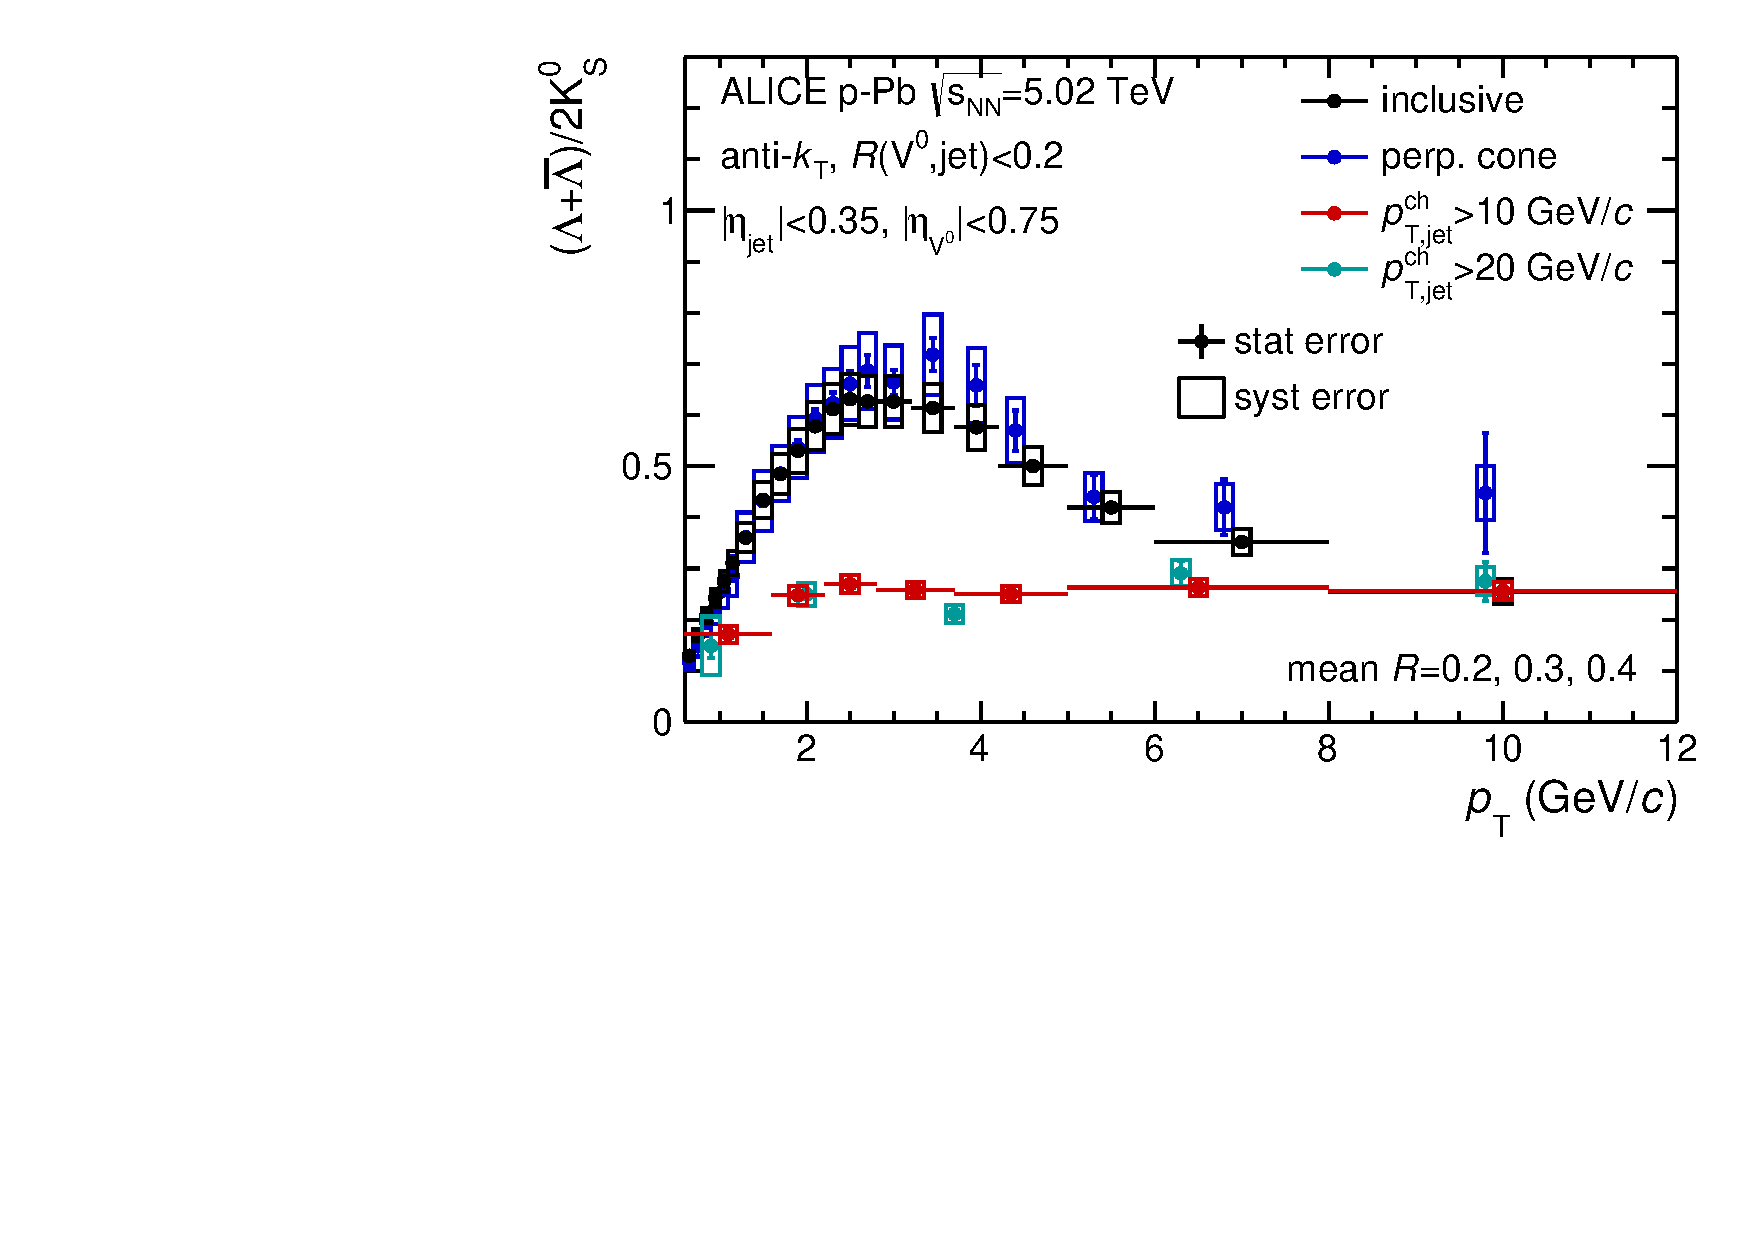
\includegraphics[width=0.47\textwidth]{cL2K_Pt_Mean_PtJE}
	\caption{\lda/\ks\ ratio in p--Pb collisions at \sqrtsnn{5.02} as a function of $R_{\Vzero-{\rm jet}}$ for three different \Vzero-particle \pt\ selections associated with charged jets with $\ptch>10~\gevc$ (left) and as a function of \Vzero-particle \pt\ associated with charged jets with $\ptch>10~\gevc$ and $20~\gevc$ together with that in inclusive and PC distribution (right). For more details see legend.}
	\label{fig:L2Kratio}
	\label{fig:LKR}
\end{figure}

\subsection{Discussion}
%% \ask{the following is to be reworked or removed all together - it is a comment and not altering any of the conclusions:}

Selecting hard scatterings according to the jet energy carried exclusively by the primary charged particles induces biases and inefficiencies in selection of the parton showers.
The bias is related to the probabilistic process of fragmentation and hadronization.
The analysis presented here tags only parton showers fragmenting into a configuration of hadrons that produce charged particle jet with $\ptch>10~\gevc$ with a given $R$ with a finite efficiency.
Therefore, there can be cases of \Vzero\ particles that originated from a parton shower but were rejected in the analysis based on the energy carried only by the primary charged particles.
The same analysis performed using PYTHIA event generator shows that the most probable \pt\ of the full jet with $R=0.4$ is larger by about 40\% as compared to the \ptch.
Moreover, since the daughters of the \Vzero\ particles are not included in the jet energy calculation there are cases of jets containig \Vzero\ particles but not included in the JC selection.
On the other hand, the right panel of Fig. \ref{fig:L2Kratio} shows that the inclusive \lda/\ks\ ratio at high-\pt\ is fully consistent with the ratio from particles associated to jets in this analysis. This corroborates the conclusion that the absence of the baryon/meson enhancement in jets made with the charged jets alone holds for all energetic parton showers and hadron configurations within jets.

%%%%%%%%%%%%%%%%%%%%%%%%%%%%%%%%%%%%%%%%%%%%%%%%%%%%%%%%%%%%%%%%%%%%%

\section{Summary}

In conclusion, the enhancement in the $(\lda+\alda)/\ks$ ratio found in the \pPb\ and \PbPb\ collisions is not present in \pPb\ for particles associated to a hard scattering tagged by jets reconstructed from charged particles for $\ptch>10~\gevc$.
This conclusion is consistent with the measurements in \PbPb\ collisions where the relative fragmentation into hadrons at high-\pt, even in central collisions, is not modified by the medium \cite{Abelev:2013xaa,Abelev:2014laa,Adam:2015kca}.
Moreover, as the baryon/meson enhancement has been linked to the interplay of radial flow and parton recombination at intermediate-\pt\ its absence within the jet cone demonstrates that these effects are limited to the soft processes of particle production.

%\begin{enumerate}
%	\item spectra harder in jets
%	\item L/K ratio: a) different than inclusive or OC/PC/NJ/inclusive - no peak; b) consistent with vacuum within uncertainties -> UE radial flow; jets do not flow
%	%%\item mean \pt -> hint softening of jet fragments in most central collisions? - tension with 2.b
%	\item constraint on the soft-hard parton recombination (?)
%\end{enumerate}

